%% \documentclass[preprint,12pt]{Elsevier/elsarticle}
%% \documentclass[preprint,review,12pt]{Elsevier/elsarticle}
%% \documentclass[final,1p,times]{Elsevier/elsarticle}
%% \documentclass[final,1p,times,twocolumn]{Elsevier/elsarticle}
   \documentclass[final,3p, review, times]{Elsevier/elsarticle}
%% \documentclass[final,3p,times,twocolumn]{Elsevier/elsarticle}
%% \documentclass[final,5p,times]{Elsevier/elsarticle}
%% \documentclass[final,5p,times,twocolumn]{Elsevier/elsarticle}


%% ------ Custom Packages -----------
\usepackage{etex}
\usepackage{amsmath}
\usepackage{amssymb}
\usepackage{xcolor}
\usepackage{fancyvrb}
\usepackage{hyperref}
\usepackage{graphicx}
\usepackage{listings}
\usepackage{titlesec}
\usepackage{paralist}
\usepackage{multirow}
\usepackage{calc}
\usepackage{soul}  %% for highlighting text
\usepackage{pstricks,pst-node,pst-tree,pstricks-add}  %% for drawing CFG and 2D view of the lattice
\usepackage{tikz}  %% for drawing rest of the images
\usetikzlibrary{shapes, snakes, decorations.markings}
\tikzset{
  ->-/.style={
    thick,
    postaction = {decorate},
    decoration = {
      markings,
      mark = at position #1 with {
        \arrow{stealth}
      }
    }
  },
  ->-/.default = 0.5
}
\tikzset{
  -<-/.style={
    thick,
    postaction = {decorate},
    decoration = {
      markings,
      mark = at position #1 with {
        \arrow{stealth reversed}
      }
    }
  },
  -<-/.default = 0.5
}

%% ------ Custom Commands -----------
\makeatletter
\newcommand{\op}[3][\@empty]{
  \ifx\@empty#1\relax
    \ \tikz[baseline=(char.base)]{
      \node[shape=circle,draw,inner sep=0pt] (char) {$\mathtt{{#2}_{#3}}$};
    }\ 
  \else
    \ \tikz[baseline=(char.base)]{
      \node[shape=circle,draw,fill=black!90,text=white,inner sep=0pt] (char) {$\mathtt{{#2}_{#3}}$};
    }\ 
  \fi
}
\makeatother
\newlength{\depthofsumsign}
\setlength{\depthofsumsign}{\depthof{$\sum$}}
\newcommand{\nsum}[1][1.4]{
  \mathop{
    \raisebox{
      -#1\depthofsumsign+1\depthofsumsign
    }{
      \scalebox{#1}{$\displaystyle\sum$}
    }
  }
}
\titleformat*{\section}{\Large}
\newcommand{\ALPHA}{\large\boldsymbol{\alpha}\normalsize}
\newcommand{\GAMMA}{\large\boldsymbol{\gamma}\normalsize}
\DefineVerbatimEnvironment{snippet}{Verbatim}{
  frame=single,
  framerule=0.1mm,
  rulecolor=\color{gray},
  labelposition=bottomline,
  numbers=left,
  numbersep=2pt,
  numberblanklines=false,
  commandchars=\\\{\},
  framesep=2mm,
  xleftmargin=0mm,
  xrightmargin=0mm,
  label={\color{black}{\bf\snippetLabel}\color{gray}},
  codes={\catcode`$=3\catcode`^=7\catcode`_=8}
}
\hypersetup{
  pdfstartview = {FitH},
  pdffitwindow = true,
  pdfnewwindow = true,
  colorlinks   = true,
  urlcolor     = blue,
  linkcolor    = blue,
  citecolor    = cyan,
  pdfauthor    = {Dibyendu Das},
  pdfcreator   = {LaTeX},
  pdfkeywords  = {Interval Analysis, Static Analysis, Abstract Interpretation, Probabilistic Programming Language},
  pdftitle     = {Interval Analysis of Unreliable Programs},
  pdfsubject   = {Research Thesis},
  pdfpagemode  = UseNone
}
%% ------------------------------

\begin{document}

\title{
{--------------------------------------------------------------------}\\
{Interval Analysis of Unreliable Programs}\\
{--------------------------------------------------------------------}\\
{\large A thesis submitted in partial fulfillment of\\
The requirements for the degree of Master of Technology\\
in\\
Computer Science and Engineering\\}
}
\author{By\\
Dibyendu Das\\
Roll No. 14CS60R34\\
Under the supervision of\\
Prof Soumyajit Dey\\
Dept. of CSE, IIT Kharagpur\\~\\

\includegraphics[width=5cm]{logo.jpg}\\
Department of Computer Science and Engineering\\
Indian Institute of Technology, Kharagpur}
\maketitle
\clearpage

\tableofcontents

\clearpage
\phantomsection
\chapter{\LARGE\begin{center}Certification\end{center}}
{\large
This is to certify that the project entitled "\textit{Interval Analysis of Unreliable Programs}" being submitted by Dibyendu Das is a bonafide work done by him in the Department of Computer Science and Engineering, Indian Institute of Technology, Kharagpur under my supervision and guidance for M.Tech Project.}\\~\\~\\~\\~\\~\\~\\~\\~\\~\\~\\~\\~\\~\\~\\~\\~\\~
\begin{flushright}
---------------------------------------------------------------------\\~\\~
Prof. Soumyajit Dey \\~
Department of Computer Science and Engineering\\~
IIT Kharagpur\\~
\end{flushright}

\clearpage
\phantomsection
\chapter{\LARGE\begin{center}Declaration\end{center}}
{\large
This thesis is a presentation of my original research work. Wherever contributions of others are involved, every effort is made to indicate this clearly, with due reference to the literature and acknowledgement of collaborative researchand discussions. The work was done under the guidance of Prof. Soumyajit Dey, at Indian institute of Technology, Kharagpur.}\\~\\~\\~\\~\\~\\~\\~\\~\\~\\~\\~\\~\\~\\~\\~\\~\\~
\begin{flushright}
---------------------------------------------------------------------\\~\\~
Dibyendu Das\\~
Department of Computer Science and Engineering\\~
IIT Kharagpur\\~
\end{flushright}

\clearpage
\phantomsection
\chapter{\LARGE\begin{center}Acknowledgements\end{center}}
{\large This thesis is the result of the project work performed under the guidance of Prof. Soumyajit Dey at the Department of Computer Science and
Engineering of the Indian Institute of Technology, Kharagpur. I am deeply grateful to my supervisor for having given me the opportunity of working under him and guiding me seamlessly for the whole period. He gave me exposure to all the related research going on in this field, which helped me enormously. Without the help, encouragement and patient support I received from my guide, this report would never have materialized.}\\~\\~\\~\\~\\~\\~\\~\\~\\~\\~\\~\\~\\~\\~\\~\\~\\~
\begin{flushright}
---------------------------------------------------------------------\\~\\~
Dibyendu Das\\~
Department of Computer Science and Engineering\\~
IIT Kharagpur\\~
\end{flushright}

\clearpage
\phantomsection
\chapter{\LARGE\begin{center}Abstract\end{center}}
Advancement of chip technology will make futute computer chips more and more fast. But this speed gain doesn't come free of cost. There is going to be a trade-off between speed and efficiency, i.e accuracy of the computation. In order to achieve this ultra speed we'll simply have to let our computers make more mistakes in computations.

Our objective in this project is to statically analyse codes written for these kind of architecture. We have used a C-type language to model the programs written for this architecture. One example of such unreliable programs is RELY[3]. Our static analysis primarily focuses on \textit{Interval Analysis} of this sort of programs.  There are 2 types of failures of the hardware components namely: \emph{permanent failure model} (where the hardware stops on failure) and \emph{transient failure model} (where, on failure, the hardware continues with the next operations). We've only taken transient failure model into consideration.

The goal of this analysis is to be able to predict, \textbf{for each program variable at each program point, the interval/range within which it belongs with a particular certainty/confidence}. say for example, the program has $n$ variables namely $x_1,x_2\cdots x_n$. Our analysis will produce output something like $x_i=\langle[a,b],p_{ab}\rangle$ for each $i$, at every program point. This means that variable $x_i$, at that program point lines in the interval $[a,b]$ with probability $p_{ab}$.

\emph{Abstract Interpretation} is what we've based our technique on. For that we've come up with two new complete lattices (one concrete and one abstract) for our probabilistic domains and established Galois Connection between them. Right now we're only concerned for program variables storing integer values.

The major applications or this work can be \emph{calculating the success probability of the overall program}, \emph{static branch prediction} for such languages. Other application could be \emph{detection of most reliable path in the program}.
\clearpage



\section{Introduction}

As transistors get smaller, they also become less reliable. So far, computer-chip designers have been able to work around that problem, but in the future, it could mean that computers stop improving at the rate we’ve come to expect.

A third possibility, which some researchers have begun to float, is that we could simply let our computers make more mistakes. This reliability won't be a major issue in some cases. If, for instance, a few pixels in each frame of a high-definition video are improperly decoded, viewers probably won’t notice --- but relaxing the requirement of perfect decoding could yield gains in speed or energy efficiency.

Emerging high-performance architectures are anticipated to contain unreliable components that may exhibit soft errors, which silently corrupt the results of computations. Full detection and masking of soft errors is challenging, expensive, and, for some applications, unnecessary. For example, approximate computing applications such as
\begin{inparaenum}[\itshape i\upshape)]
  \item Multimedia processing,
  \item High definition video decoding,
  \item Image manipulation,
  \item Machine learning,
  \item Big data analytics
\end{inparaenum}
can often naturally tolerate soft errors.

For handling the future unreliable chips, a research group at MIT's Computer Science and Artificial Intelligence Laboratory (CSAIL) has developed a new programming framework called \textbf{RELY}\cite{carbin13} that enables software developers to specify when errors may be tolerable. The system then calculates the probability that the software will perform as it's intended.

Here, we present an amended form of the popular static analysis tool called \textbf{Range Analysis} or \textbf{Interval Analysis} for unreliable programs as such. We call it \textbf{Probabilistic Interval Analysis}. Our model is so modified as to incorporate the unreliabilities occur because of unreliable ALU and memory operations.

\section{Objective}

We propose a general abstract interpretation based method for the static analysis of programs that run on unreliable hardwares. Our method does Interval analysis for programs like these. The objectibe is to calculate the success probability of the overall program and other similar tasks like detecting the most reliable path in the program.

More formally, for a program with $n$ integer variables, we are interested in answering questions like, with what probability does each program variable lie in a range of values at each program point. In other words, goal is to find out the probability that $x_i\in[a,b]$ at program point $p_i$.

\section{Related Work}

There have already been some work on static analysis of programs with \emph{imprecise probabilistic inputs} \cite{vstte13}, which heavily relies on Dempster-Shafer structures (DSI) or P-boxes. This analyzer assumes each input value to be lying within a \textit{confidence box} $[\underline{P},\overline{P}]$. Based on this assumption it works on to perform the interval analysis of each variable at each program point.

Few more works are there that analyze programs with non-deterministic and probabilistic behavior \cite{monn01}\cite{sumit13}. Those use general abstract interpretation based method for the static analysis of programs using random generators or random inputs and also allow non-deterministic inputs, not necessarily following a random distribution.

Our work is orthogonal to all these as we're concerned with the imprecision seeded into the hardware rather than in input. So, in my case inputs come from reliable sources with fully reliable values.

\section{Unreliable Programs}

Following is an example program snippet and its corresponding \textbf{C}ontrol \textbf{F}low \textbf{G}raph for RELY like programming languages.

\begin{minipage}[b]{0.40\linewidth}
\centering
\begin{lstlisting}[mathescape]
//$v_0$
x $=_\bullet$ 0
//$v_1$
while (x $<_\bullet$ 10) // $v_2$
    x $=_\bullet$ x $+_\bullet$ 3
//$v_3$
\end{lstlisting}
\end{minipage}
\rule[42mm]{4mm}{.1pt}\rule[-2.5mm]{1pt}{50mm}\rule[42mm]{4mm}{.1pt}\raisebox{41.2mm}{$>$ CFG}
\hspace{0.2\linewidth}
\begin{minipage}[b]{0.40\linewidth}
$
\psmatrix[colsep=2.5cm,rowsep=1.5cm,mnode=circle]
v_0\\
v_1&v_3\\
v_2
\psset{arrowscale=2}
\everypsbox{\scriptstyle}
\ncline{->}{1,1}{2,1}>{x\ =_\bullet\ 0}
\ncline{->}{2,1}{2,2}^{x\ \geq_\bullet\ 10}
\ncline{->}{2,1}{3,1}>{x\ \leq_\bullet\ 9}
\ncarc[arcangle=-45]{<-}{2,1}{3,1}<{x\ =_\bullet\ x\ +_\bullet\ 3}
\endpsmatrix
$
\end{minipage}

\centerline{Figure 1: Example program.}

Here each operation is probabilistic i.e each operation produces correct values with some probability. Unreliable operators are denoted by the corresponding operator followed by a \textit{subscript bullet} ($\bullet$). Each operator has a success probability associated with it i.e the operator succeeds and produces correct result with a predefined probability. These probability values are set by the hardware manufacturer of the chip. Upon failure the probabilistic operators take random values from their corresponding domains. For arithmatic operators this domain is $\mathbb{Z}\cap[\mathtt{MININT},\mathtt{MAXINT}]$, for boolean operators it is $\{true, false\}$ etc. We define the success probabilities of some of the operators as follows :\\

\centerline{
  \begin{tabular}{c|c|c|c}
    \hline
    \multirow{2}{*}{Operator} & Probability of successful execution & \multirow{2}{*}{Failure probability} & \multirow{2}{*}{Domain of operation} \\
    & (set by hardware manufacturer) & & \\ \hline
    $+_\bullet$ & $Pr(+_\bullet)$ & $1-Pr(+_\bullet)$ & \multirow{5}{*}{$\big\{a\in\mathbb{Z}\quad|\quad\mathtt{MININT}\leq a\leq\mathtt{MAXINT}\big\}$} \\
    $-_\bullet$ & $Pr(-_\bullet)$ & $1-Pr(-_\bullet)$ & \\
    $\times_\bullet$ & $Pr(\times_\bullet)$ & $1-Pr(\times_\bullet)$ & \\
    $\div_\bullet$ & $Pr(\div_\bullet)$ & $1-Pr(\div_\bullet)$ & \\
    $=_\bullet$ & $Pr(Wr)$ & $1-Pr(Wr)$ & \\ \hline
    $>_\bullet$ & $Pr(>_\bullet)$ & $1-Pr(>_\bullet)$ & \multirow{2}{*}{$\big\{true,\ false\big\}$} \\
    $\geq_\bullet$ & $Pr(\geq_\bullet)$ & $1-Pr(\geq_\bullet)$ & \\
  \end{tabular}
}
\centerline{$\vdots$}

\noindent E.g: This program statement \\ \centerline{$\sigma : x\ =_\bullet\ x\ +_\bullet\ 3$} \\ involves 3 probabilistic operations namely Read (\textbf{Rd}) of the variable $x$, Add (\textbf{+}) \& Write (\textbf{Wr}) to the variable $x$. So, the probability that $\sigma$ executes successfully is $\quad Pr(Rd)\cdot Pr(+_\bullet)\cdot Pr(Wr)$. Now we compute the probability with which program variable $x$ holds correct value after the execution of $\sigma$.

These three operations are independent of each other. Corresponding to three operations we have three events namely:

\begin{itemize}
\item A: \textbf{Read} executes successfully.
\item B: \textbf{Add} ($+_\bullet$) executes successfully.
\item C: \textbf{Write} executes successfully.
\end{itemize}

$\therefore\qquad Pr(A)=Pr(Rd),\quad Pr(B)=Pr(+_\bullet)\quad\text{and}\quad Pr(C)=Pr(Wr)$.

All three events are pairwise independent but none of them are mutually exclusive.\\


\def\firstcircle{(0,0) circle (1.5cm)}
\def\secondcircle{(60:2cm) circle (1.5cm)}
\def\thirdcircle{(0:2cm) circle (1.5cm)}
\centerline{
\begin{tikzpicture}
\begin{scope}[shift={(3cm,-5cm)}, fill opacity=0.5]
\fill[gray] \firstcircle;
\fill[lightgray] \secondcircle;
\fill[white] \thirdcircle;
\draw \firstcircle node[below left] {$A$};
\draw \secondcircle node [above] {$B$};
\draw \thirdcircle node [below right] {$C$};
\end{scope}
\end{tikzpicture}
}


After $\sigma$ is executed the variable $x$ will hold the desired value with probability
$$\displaystyle Rel_{cur}(x) = Rel_{prev}(x)\cdot\left(Pr(Rd) + \frac{1-Pr(Rd)}{\mathtt{MAXINT}-\mathtt{MININT}+1}\right)\cdot\left(Pr(+_\bullet) + \frac{1-Pr(+_\bullet)}{\mathtt{MAXINT}-\mathtt{MININT}+1}\right)\cdot\left(Pr(Wr) + \frac{1-Pr(Wr)}{\mathtt{MAXINT}-\mathtt{MININT}+1}\right)$$

Where, \underline{$Rel_{prev}(x)$} is the probability with which variable $x$ holds the correct value just before this statement is executed.

We are interested in static analysis of these type of probabilistic programs by employing the theory of abstraction using Galois Connection (GC).

\section{The Probabilistic Concrete Domain, $L$}

From the above arguments we can infer that in the concrete domain each possible program state is associated with some probability. We represent program state as a tuple of set of values and its associated probability. Set of all possible program states is thus represented by

\centerline{
  $\mathbb{Z}_p=\Big\{\langle a,p_a\rangle\quad\big|\quad a\in\mathbb{Z}, p_a\in\mathbb{R}, \mathtt{MININT}\leq a\leq\mathtt{MAXINT}, 0\leq p_a\leq1\Big\}$
}

Throughout our discussion we assume that our program variables take values between $\mathbf{\mathtt{MININT}}$ and $\mathbf{\mathtt{MAXINT}}$ (including both). $\langle a_i,p_{a_i}\rangle$ denotes that at a particular program point $v_i$, variable $x_i$ takes the value $a_i$ with probability $p_{a_i}$. For $1\leq i\leq n$, We define two utility functions as follows :
\begin{align}
  \mathbf{val}\bigg(\Big(\langle a_1,p_{a_1}\rangle,\langle a_2,p_{a_2}\rangle\cdots\langle a_n,p_{a_n}\rangle\Big),i\bigg)=a_i\label{eq:val}\\
  \mathbf{prob}\bigg(\Big(\langle a_1,p_{a_1}\rangle,\langle a_2,p_{a_2}\rangle\cdots\langle a_n,p_{a_n}\rangle\Big),i\bigg)=p_{a_i}\label{eq:prob}\\
\end{align}

In this case, the concrete domain $L$ is a subset of the power set of $\mathbb{Z}_p$. For program with a single integer variable, the concrete domain is $L=\Big\{S\in2^{^{\mathbb{Z}_p}}\ \Large:\ \normalsize S\ \text{is finite}\bigwedge\big|\big\{\mathbf{val}(t)\ |\ \forall t\in S\big\}\big|=\big|S\big|\Big\}$\footnote{This way we ensure that values in each element of $L$ are unique. For example, $\Big\{\langle a,p_a\rangle,\ \langle b,p_b\rangle\Big\}\in L$ but $\Big\{\langle a,p_a\rangle,\ \langle b,p_{b_1}\rangle,\ \langle b,p_{b_2}\rangle\Big\}\notin L$}, set of all feasible sets of program states. In general, for program with $n$ integer variables, this concrete domain will be : $\displaystyle\bigwedge_i \forall S_i\in L,\quad\Big\{S_1\times S_2\times\cdots\times S_n\Big\}=L_n.$

We define a partial order $\sqsubseteq_L$ on $L$ as follows :

\centerline{$\forall A,B\in L\qquad A\sqsubseteq_L B$}
iff
\begin{enumerate}[i)]
\item $\Big\{\mathbf{val}(t)\ \big|\ \forall t\in A\Big\}\subseteq\Big\{\mathbf{val}(t)\ \big|\ \forall t\in B\Big\}$
\item $\forall t_a\in A,\ \forall t_b\in B\quad\bigg(\Big(\mathbf{val}(t_a)=\mathbf{val}(t_b)\Big)\Rightarrow\Big(\mathbf{prob}(t_a)\geq\mathbf{prob}(t_b)\Big)\bigg)$
\end{enumerate}
all the above conditions hold simultaneously. As an example,\\
\centerline{
  $\Big\{\langle a_1,p_{a_1}\rangle,\ \langle a_2,p_{a_2}\rangle\ \cdots\ \langle a_n,p_{a_n}\rangle\Big\}\sqsubseteq_L\Big\{\langle a_1,p'_{a_1}\rangle,\ \langle a_2,p'_{a_2}\rangle\ \cdots\ \langle a_m,p'_{a_m}\rangle\Big\}\qquad$ iff
}
\centerline{
  $n\leq m, \text{so that\ }\big\{a_1,a_2\ \cdots\ a_n\big\}\subseteq\big\{a_1,a_2\ \cdots\ a_m\big\}\qquad$and$\qquad\displaystyle\bigwedge_n \big(p_{a_i}\geq p'_{a_i}\big)$
}

$(L,\ \sqsubseteq_L)$ is a \textbf{poset}, proof of which is given in \ref{app:concrete_partial}. To show this poset to be a \textbf{lattice}, we need to show that for any two elements in $L$ there exist a unique infimum and a unique supremum. More formally
\begin{align*}
  \forall x,y\in L\ \ \Bigg(\exists L_{lub}\in\Big\{u\in L\ \ \big|\ \ (x\sqsubseteq_L u)\land(y\sqsubseteq_L u)\Big\}\ &s.t\ \bigg(\forall z\ \ \Big(z\in\Big\{u\in L\ \ \big|\ \ (x\sqsubseteq_L u)\land(y\sqsubseteq_L u)\Big\} \Rightarrow L_{lub}\sqsubseteq_L z\Big)\bigg)\\
  &\bigwedge\\
  \exists L_{glb}\in\Big\{l\in L\ \ \big|\ \ (l\sqsubseteq_L x)\land(l\sqsubseteq_L y)\Big\}\ &s.t\ \bigg(\forall z\ \ \Big(z\in\Big\{l\in L\ \ \big|\ \ (l\sqsubseteq_L x)\land(l\sqsubseteq_L y)\Big\} \Rightarrow z\sqsubseteq_L L_{glb}\Big)\bigg)\Bigg)
\end{align*}
where $L_{lub}$ is the least upper bound and $L_{glb}$ is the greatest lower bound of $x$ and $y$ in $L$. We now define the least upper bound or $l.u.b$, $\displaystyle\bigsqcup_L$ and the greatest lower bound or $g.l.b$, $\displaystyle\bigsqcap^L$ for any two elements $A$ and $B$ of $L$ as follows.

\begin{align}
    A\ \bigsqcup_L\ B\quad=\quad&\Big\{t_a\ \big|\  t_a\in A\bigwedge \mathbf{val}(t_a)\notin \big\{\mathbf{val}(t_b)\ |\ t_b\in B\big\}\Big\}\ \bigcup\ \Big\{t_b\ \big|\  t_b\in B\bigwedge \mathbf{val}(t_b)\notin \big\{\mathbf{val}(t_a)\ |\ t_a\in A\big\}\Big\}\ \bigcup&\nonumber\\
    &\qquad\qquad\qquad\qquad\Big\{\big\langle\mathbf{val}(t_a),\mathbf{min}\big(\mathbf{prob}(t_a),\mathbf{prob}(t_b)\big)\big\rangle\ \big|\  t_a\in A, t_b\in B\bigwedge \mathbf{val}(t_a)=\mathbf{val}(t_b)\Big\}&\label{eq:lub_L}\\
    A\ \bigsqcap^L\ B\quad=\quad&\Big\{\big\langle\mathbf{val}(t_a),\mathbf{max}\big(\mathbf{prob}(t_a),\mathbf{prob}(t_b)\big)\big\rangle\ \big|\  t_a\in A, t_b\in B\bigwedge \mathbf{val}(t_a)=\mathbf{val}(t_b)\Big\}&\label{eq:glb_L}
\end{align}

Soundness of these definitions is proved in \ref{app:concrete_ub}. Greatest and least element of this lattice $(L,\ \sqsubseteq_L)$ are $\top_L$ and $\bot_L$ respectively, where

$\top_L=\big\{\langle a,0\rangle\ \big|\ a\in[\mathtt{MININT},\mathtt{MAXINT}]\big\}=\big\{\langle\mathtt{MININT},0\rangle\ \cdots\ \langle -1,0\rangle,\langle 0,0\rangle,\langle 1,0\rangle\ \cdots\ \langle\mathtt{MAXINT},0\rangle\big\}$

$\bot_L=\big\{\ \big\}$

The \textbf{Hasse Diagram} of lattice $(L,\sqsubseteq_L)$ can be found in \ref{app:concrete_hasse}. $\forall S\subseteq L,\quad S$ has a unique $l.u.b$ and $g.l.b$ in $L$. Hence $L$ is a complete lattice.

Next, we shall define a function on $L_n$ called the \textit{strongest post-condition function}\cite{lara13}.

Consider $P$ to be a predicate defined over program variables. Alternatively, we can also think of $P$ as a set of possible program states which satisfy the relation $P$. For example, $p=(\langle5,p_1\rangle)\equiv[x=5]$ is a program state ($p_1$ is a place-holder here) and $P:[x>10]$ is a predicate such that $p\notin P$. Similarly, consider a program with three integer variables $x,\ y$ and $z$ such that $p=\big(\langle5,p_1\rangle,\langle10,p_2\rangle,\langle10,p_3\rangle\big)\equiv[x=5,\ y=10,\ z=10]$ and $p'=\big(\langle15,p'_1\rangle,\langle0,p'_2\rangle,\langle1,p'_3\rangle\big)\equiv[x=15,\ y=0,\ z=1]$ are two program states. Given a predicate $P:[x+y\geq z]$, we may observe that both $p,p'\in P$. Let $P$ denote a (pre-condition) predicate which is true before the execution of some program statement $S$. Strongest post condition (sp) is a function which takes as argument a program statement $S$ (or a sequence of statements) and a predicate $P$ and returns the strongest predicate that holds after executing $S$ from any program state which satisfies $P$. It is strongest in the sense that for any other such predicate $Q$ which holds for any state resulting from execution of $S$ given $P$, we shall always have $sp(P,S)\Rightarrow Q$ (implies $Q$) or in a set theoretic notation $sp(P,S)\subseteq Q$. As example, we consider next arithmetic expressions (with assignment) and logical expressions as examples of $S$.

We assume that there are $n$ variables in the program, namely, $x_1,x_2\cdots x_n$.

\begin{flalign}
  &sp\Big(P,\ x_{i_f} =_\bullet x_{i_1} \op[prob]{A}{2} x_{i_2} \op[prob]{A}{3} \cdots \op[prob]{A}{k} x_{i_k}\Big)&&&\nonumber\\
  &=\left\{\Big(\left\langle a_1,p_1\right\rangle,\left\langle a_2,p_2\right\rangle\cdots\left\langle a_n,p_n\right\rangle\Big)\ \middle|\ \exists t\in P'\left(a_{i_f}=\mathbf{val}(t,i_f)\ \bigwedge\ p_{i_f}=\left(\nsum[2]_{\forall t'\in P',\ \mathbf{val}(t',i_f)=\mathbf{val}(t,i_f)}{\mathbf{prob}(t',i_f)}\right)\ \cdot\right.\right.&&&\nonumber\\
  &\quad\left(Pr(Wr)+\frac{1-Pr(Wr)}{\mathtt{MAXINT}-\mathtt{MININT}+1}\right)\cdot\left(Pr(Rd) + \frac{1-Pr(Rd)}{\mathtt{MAXINT}-\mathtt{MININT}+1}\right)^l\cdot\prod_{j=2}^k\left(Pr\left(\op[prob]{A}{j}\right)+\frac{1-Pr\left(\op[prob]{A}{j}\right)}{\mathtt{MAXINT}-\mathtt{MININT}+1}\right)\ \bigwedge&&&\nonumber\\
  &\qquad\qquad\forall j\in\mathbb{N}\setminus\{i_f\}\left(j\leq n\ \Rightarrow a_j=\mathbf{val}(t,j)\ \bigwedge\ p_j=\mathbf{prob}(t,j)\right)\Bigg)\Bigg\}&&&\label{eq:sp_arith}\\
  &\text{where,}\ l=\Big|\big\{i_k\ |\ x_{i_k}\text{ is a variable}\big\}\Big|\qquad\text{and}&&&\nonumber\\
  &P'=\left\{\Big(\left\langle a_1,p_1\right\rangle,\left\langle a_2,p_2\right\rangle\cdots\left\langle a_n,p_n\right\rangle\Big)\ \middle|\ \exists t\in P\left(a_{i_f}=\left(v(t,x_{i_1}) \op{A}{2} v(t,x_{i_2}) \op{A}{3} \cdots \op{A}{k} v(t,x_{i_k})\right)\ \bigwedge\ p_{i_f}=\prod_{j=1}^k p(t,x_{i_j})\ \bigwedge\right.\right.&&&\nonumber\\ 
  &\qquad\qquad\forall j\in\mathbb{N}\setminus\{i_f\}\left(j\leq n\ \Rightarrow a_j=\mathbf{val}(t,j)\ \bigwedge\ p_j=\mathbf{prob}(t,j)\right)\Bigg)\Bigg\}&&&\nonumber\\
  &sp\left(P,\ \left(x_{i_1} \op[prob]{A}{i_2} x_{i_2} \op[prob]{A}{i_3} \cdots \op[prob]{A}{i_k} x_{i_k}\right)\ \op[prob]{C}{}\ \left(x_{j_1} \op[prob]{A}{j_2} x_{j_2} \op[prob]{A}{j_3} \cdots \op[prob]{A}{j_m} x_{j_m}\right)\right)&&&\nonumber\\
  &=\left\{\Big(\left\langle a_1,p_1\right\rangle,\left\langle a_2,p_2\right\rangle\cdots\left\langle a_n,p_n\right\rangle\Big)\ \middle|\ \exists t\in P\left(\forall j\in\mathbb{N}\left(j\leq n\ \Rightarrow a_j=\mathbf{val}(t,j)\ \bigwedge\ p_j=\left(Pr(Rd) + \frac{1-Pr(Rd)}{\mathtt{MAXINT}-\mathtt{MININT}+1}\right)^l\cdot\right.\right.\right.&&&\nonumber\\
  &\quad\left.\left.\left.\left(Pr\left(\op[prob]{C}{}\right)+\frac{1-Pr\left(\op[prob]{C}{}\right)}{2}\right)\cdot\prod_{j=2}^k\left(Pr\left(\op[prob]{A}{i_j}\right)+\frac{1-Pr\left(\op[prob]{A}{i_j}\right)}{\mathtt{MAXINT}-\mathtt{MININT}+1}\right)\cdot\prod_{i=2}^m\left(Pr\left(\op[prob]{A}{j_i}\right)+\frac{1-Pr\left(\op[prob]{A}{j_i}\right)}{\mathtt{MAXINT}-\mathtt{MININT}+1}\right)\cdot\right.\right.\right.&&&\nonumber\\
  &\qquad\mathbf{prob}(t,j)\Bigg)\ \bigwedge\ \left(v(t,x_{i_1}) \op{A}{i_2} v(t,x_{i_2}) \op{A}{i_3} \cdots \op{A}{i_k} v(t,x_{i_k})\right)\ \op{C}{}\ \left(v(t,x_{j_1}) \op{A}{j_2} v(t,x_{j_2}) \op{A}{j_3} \cdots \op{A}{j_m} v(t,x_{j_m})\right)\Bigg)\Bigg\}&&&\label{eq:sp_cond}\\
  &\text{where,}\ l=\Bigg|\Bigg\{x\in\Big\{x_{i_1},x_{i_2}\cdots x_{i_k}\Big\}\bigcup\Big\{x_{j_1},x_{j_2}\cdots x_{j_m}\Big\}\Bigg| x\text{ is a variable}\Bigg\}\Bigg|&&&\nonumber
\end{flalign}
In the above equations,
\begin{flalign}
  &v(t,x_i)=\begin{cases}
  		\mathbf{val}(t,i)       & \quad \text{if } x_i \text{ is a variable}\\
  		x_i=C  & \quad \text{if } x_i \text{ is a constant, say } C\\
  \end{cases}\qquad\text{and}\qquad
  p(t,x_i)=\begin{cases}
  		\mathbf{prob}(t,i)       & \quad \text{if } x_i \text{ is a variable}\\
  		1  & \quad \text{if } x_i \text{ is a constant}\\
  \end{cases}&&&\nonumber\\
  &\forall i,\quad\op[prob]{A}{i} \text{ is a probabilistic arithmatic operation}\quad\text{and}\quad\op{A}{i} \text{ is a deterministic arithmatic operation.}&&&\nonumber\\
  &\text{i.e}\quad\op[prob]{A}{i}\in\{+_{\bullet},-_{\bullet},\times_{\bullet},\div_{\bullet},\%_{\bullet},\cdots\}\quad\op{A}{i}\in\{+,-,\times,\div,\%,\cdots\}&&&\nonumber\\
  &\op[prob]{C}{} \text{ is a probabilistic comparison operation}\quad\text{and}\quad\op{C}{} \text{ is a deterministic comparison operation.}&&&\nonumber\\
  &\text{i.e}\quad\op[prob]{C}{}\in\{<_{\bullet},>_{\bullet},\geq_{\bullet},\leq_{\bullet},==_{\bullet},\neq_{\bullet}\}\quad\op{C}{}\in\{>,<,\geq,\leq,==,\neq\}&&&\nonumber
\end{flalign}
\begin{flalign}
  &sp\Big(P,\ x =_\bullet 0\Big)&=&\left\{\left(\left\langle0,\ Pr(Wr)+\frac{1-Pr(Wr)}{\mathtt{MAXINT}-\mathtt{MININT}+1}\right\rangle\right)\right\}&\label{eq:sp1}\\
  &sp\Big(P,\ x =_\bullet x +_\bullet 3\Big)&=&\left\{\left(\left\langle\mathbf{val}(t,1) + 3,\ \mathbf{prob}(t,1)\cdot\left(Pr(Rd) + \frac{1-Pr(Rd)}{\mathtt{MAXINT}-\mathtt{MININT}+1}\right)\cdot\right.\right.\right.\nonumber&\\
  &&&\quad\left.\left.\left.\left(Pr(+_\bullet) + \frac{1-Pr(+_\bullet)}{\mathtt{MAXINT}-\mathtt{MININT}+1}\right)\cdot\left(Pr(Wr) + \frac{1-Pr(Wr)}{\mathtt{MAXINT}-\mathtt{MININT}+1}\right)\right\rangle\right)\ \middle|\ t\in P\right\}&\label{eq:sp2}\\
  &sp\Big(P,\ x \leq_\bullet 9\Big)&=&\left\{\left(\left\langle\mathbf{val}(t,1),\ \mathbf{prob}(t,1)\cdot\left(Pr(\leq_\bullet) + \frac{1-Pr(\leq_\bullet)}{2}\right)\right\rangle\right)\ \middle|\ t\in P\bigwedge\mathbf{val}(t,1)\leq9\right\}&\label{eq:sp3}\\
  &sp\Big(P,\ x \geq_\bullet 10\Big)&=&\left\{\left(\left\langle\mathbf{val}(t,1),\ \mathbf{prob}(t,1)\cdot\left(Pr(\geq_\bullet) + \frac{1-Pr(\geq_\bullet)}{2}\right)\right\rangle\right)\ \middle|\ t\in P\bigwedge\mathbf{val}(t,1)\geq 10\right\}\label{eq:sp4}&
\end{flalign}

and so on \ldots

Here, P is a set of program states of the form $\big\{\big<a,\ p_a\big>\big\}$, with unique $a$'s, i.e $P\in L$.

Further, for any program $\sigma,\ sp\big(P = \bot_L = \{\ \},\ \sigma\big) = \bot_L= \{\ \}$. If the predicate P defines a relation which is not satisfied by any possible program state, or speaking set theoretically if P is an empty set, then it is not possible for $\sigma$ to execute at all since there is no state to start from. Thus the set of states reachable is also empty. Hence, the strongest post-condition is the empty set.

Using the notion of $sp$, we are interested in computing the set of reachable program states for every program point which is known as \textbf{\textit{collecting semantics}}. For each program point $v_i$, let $g_i$ denotes the set of reachable program states. We can consider these collection of program states, $\big(g_i\big)$ as \textbf{pre-condition} predicates for the succeeding program statement. In that case, they are linked by $sp$ to give the following system of equation.

\begin{tabular}{lcl}
$g_0$ & = & $\Big\{\big\langle a,\ 1\big\rangle\ \big|\ \forall a\in\mathbb{Z}\bigwedge\mathtt{MININT}\leq a\leq\mathtt{MAXINT}\Big\}$ \\
$g_1$ & = & $\displaystyle sp\big(g_0,\ x =_\bullet 0\big)\bigsqcup_L sp\big(g_2, x =_\bullet x +_\bullet 3\big)$ \\
$g_2$ & = & $sp\big(g_1,\ x \leq_\bullet9\big)$ \\
$g_3$ & = & $sp\big(g_1,\ x \geq_\bullet10\big)$ \\
\end{tabular}\\

We can derive an overall function $\mathcal{F}$,
$$\mathcal{F}\big(g_0,\ g_1,\ g_2,\ g_3\big) = \Big(g_0,\ sp\big(g_0,\ x =_\bullet 0\big)\bigsqcup_L sp\big(g_2,\ x =_\bullet x +_\bullet 3\big),\ sp\big(g_1,\ x \leq_\bullet 9\big),\ sp\big(g_1,\ x \geq_\bullet 10\big)\Big)$$
that maps each $g_i$ to new values of $g_i$ iteratively. The least fixed point of $\mathcal{F}$ is the final solution. We can arrive at the solution by computing the sequence, $\mathcal{F}^n\big(\bot_L,\ \bot_L,\ \bot_L,\ \bot_L\big)$\ starting with the least elements, i.e. the empty sets.

For the sake of the example we assume all the success probabilities to be $1-10^{-2}$, i.e $Pr(+_\bullet)=Pr(-_\bullet)=Pr(Rd)=Pr(Wr)=Pr(\leq_\bullet)=\quad\cdots\quad=1-10^{-2}$ and value of $\mathtt{MININT}$ and $\mathtt{MAXINT}$ to be $-32768$ and $32767$ respectively. Therefore, $\displaystyle\quad\left(Pr(+_\bullet)+\frac{1-Pr(+_\bullet)}{\mathtt{MAXINT}-\mathtt{MININT}+1}\right)=0.9900001526=x\quad\text{and}\quad\left(Pr(\leq_\bullet)+\frac{1-Pr(\leq_\bullet)}{2}\right)=0.995=y\text{ (say)}$

Solving iteratively would give us a solution as follows

\noindent
$
\bigg(\bot_L,\ \bot_L,\ \bot_L,\ \bot_L\bigg)\ \to\ 
\bigg(\Big\{\big\langle a,\ 1\big\rangle\ \big|\ \forall a\in\mathbb{Z}\bigwedge\mathtt{MININT}\leq a\leq\mathtt{MAXINT}\Big\},\ \bullet,\ \bullet,\ \bullet\bigg)\ \to\ 
\bigg(\bullet,\ \Big\{\big\langle 0,\ x\big\rangle\Big\},\ \bullet,\ \bullet\bigg)\ \to
$\\
$
\bigg(\bullet,\ \bullet,\ \Big\{\big\langle 0,\ xy\big\rangle\Big\},\ \bullet\bigg)\ \to\ 
\bigg(\bullet,\ \Big\{\big\langle 0,\ x\big\rangle,\big\langle 3,\ x^4y\big\rangle\Big\},\ \bullet,\ \bullet\bigg)\ \to\ 
\bigg(\bullet,\ \bullet,\ \Big\{\big\langle 0,\ xy\big\rangle,\big\langle 3,\ x^4y^2\big\rangle\Big\},\ \bullet\bigg)\ \to\ 
$\\
$
\bigg(\bullet,\ \Big\{\big\langle 0,\ x\big\rangle,\big\langle 3,\ x^4y\big\rangle,\big\langle 6,\ x^7y^2\big\rangle\Big\},\ \bullet,\ \bullet\bigg)\ \to\ 
\bigg(\bullet,\ \bullet,\ \Big\{\big\langle 0,\ xy\big\rangle,\big\langle 3,\ x^4y^2\big\rangle,\big\langle 6,\ x^7y^3\big\rangle\Big\},\ \bullet\bigg)\ \to\ 
$\\
$
\bigg(\bullet,\ \Big\{\big\langle 0,\ x\big\rangle,\big\langle 3,\ x^4y\big\rangle,\big\langle 6,\ x^7y^2\big\rangle,\big\langle 9,\ x^{10}y^3\big\rangle\Big\},\ \bullet,\ \bullet\bigg)\ \to\ 
\bigg(\bullet,\ \bullet,\ \Big\{\big\langle 0,\ xy\big\rangle,\big\langle 3,\ x^4y^2\big\rangle,\big\langle 6,\ x^7y^3\big\rangle,\big\langle 9,\ x^{10}y^4\big\rangle\Big\},\ \bullet\bigg)\ \to\ 
$\\
$
\bigg(\bullet,\ \Big\{\big\langle 0,\ x\big\rangle,\big\langle 3,\ x^4y\big\rangle,\big\langle 6,\ x^7y^2\big\rangle,\big\langle 9,\ x^{10}y^3\big\rangle,\big\langle 12,\ x^{13}y^4\big\rangle\Big\},\ \bullet,\ \bullet\bigg)\ \to\ 
\bigg(\bullet,\ \bullet,\ \bullet,\ \Big\{\big\langle 12,\ x^{13}y^5\big\rangle\Big\}\bigg)
$\\
       
The '$\bullet$' indicates, repetition of value from previous iteration. The overall solution is therefore

$\bigg($

$\qquad\Big\{\big\langle a,\ 1\big\rangle\ \big|\ \forall a\in\mathbb{Z}\bigwedge-32768\leq a\leq32767\Big\},
$

$\qquad\Big\{\big\langle 0,\ 0.9900001526\big\rangle,\big\langle 3,\ 0.955793619\big\rangle,\big\langle 6,\ 0.922768992\big\rangle,\big\langle 9,\ 0.890885433\big\rangle,\big\langle 12,\ 0.860103516\big\rangle\Big\},
$

$\qquad\Big\{\big\langle 0,\ 0.985050152\big\rangle,\big\langle 3,\ 0.951014651\big\rangle,\big\langle 6,\ 0.918155147\big\rangle,\big\langle 9,\ 0.886431006\big\rangle\Big\},
$

$\qquad\Big\{\big\langle 12,\ 0.855802998\big\rangle\Big\}
$

$\bigg)$

In general, we may need infinite number of iterations to converge. This is because the height of the lattice $L$ is $\infty$.


\section{The Probabilistic Interval Abstract Domain, $M$}

In this domain, $M$, the elements are of the form of tuples, $\langle[a,b],p_{ab}\rangle$, i.e with each interval there is a corresponding probability. Program variables are assigned these tuples at different program points instead of set of concrete values. E.g: program variable $x_i$ takes value $\langle[a,b],p_{ab}\rangle$ at a particular program point $v_i$, signifies that value of $x_i$ lies in the interval $[a,b]$ at that program point with probability $p_{ab}$.

We define a utility function \underline{$\mathit{p.m.f}$} (probability mass of an interval) :
\begin{equation}
\label{eq:pmf}
p.m.f\Big(\langle[a,b],p_{ab}\rangle\Big)=\frac{p_{ab}}{b-a+1}
\end{equation}

We now define a binary relation $\sqsubseteq_M$ on this set of abstract values, $M$. Before doing that we recall the case as it was with trivial Interval Abstract Domain\cite{nielson99}. Two intervals are related to each other by a binary relation $\sqsubseteq_{int}$ iff one interval is contained in the other.
\begin{equation}\label{eq:interval_def}
[a,\ b]\sqsubseteq_{int}[c,\ d]\iff (c\leq a)\land (b\leq d)
\end{equation}

Intuitively we lose precision in the interval that comes higher in the order.

Similar intuition is applicable in defining $\sqsubseteq_M$ on \textbf{Probabilistic Interval Abstract Domain} also. Two elements of $M$ are related by $\sqsubseteq_M$ if we lose precision in the element that comes higher in the order. Here, by precision we mean the \textit{accuracy (probability mass)} with which we can determine whether a program variable takes its values from the corresponding interval. For example, if one element $\langle[a,b],p_{ab}\rangle$ is more precise than another $\langle[a',b'],p'_{ab}\rangle$, this means that, with \textit{more accuracy (higher probability mass)} we can determine that program varuiable $x_i$ (say) takes its values from interval $[a,b]$ than it takes values from $[a',b']$.

We define,

\centerline{$\langle[a,b],p_{ab}\rangle\sqsubseteq_M\langle[c,d],p_{cd}\rangle$}
iff
\begin{enumerate}[i)]
\item $[a,b]\sqsubseteq_{int}[c,d]$
\item $p.m.f\Big(\langle[a,b],p_{ab}\rangle\Big)\geq\ p.m.f\Big(\langle[c,d],p_{cd}\rangle\Big)$
\end{enumerate}
all the above conditions hold simultaneously. So, clearly tuples whose intervals aren't related by $\sqsubseteq_{int}$ will not partake in $\sqsubseteq_M$.

$\sqsubseteq_M$ is a \textbf{partial order relation}. For its proof please refer to \ref{app:interval_partial}. Formal definition of the \textbf{Probabilistic Interval Abstract Domain}, $M$, is :

$M=\big\{\langle[a,b],p_{ab}\rangle\ \ |\ \ a,b\in\mathbb{Z}, p_{ab}\in\mathbb{R}, \mathtt{MININT}\leq a\leq b\leq\mathtt{MAXINT}, 0\leq p_{ab}\leq1\big\}\ \bigcup\ \big\{\perp_M\big\}$\\
where $\perp_M$ is the least element of $M$. $\bot_M=\langle[\ ],1\rangle$ i.e the tuple of empty interval and probability 1. For $n$ number of program variables this domain will be $M^n$.

The poset $(M,\ \sqsubseteq_M)$ is a \textbf{lattice}. For that we show that for any two elements in $M$ there exist a unique infimum and a unique supremum. We now define the least upper bound or $l.u.b$, $\displaystyle\bigsqcup_M$ and the greatest lower bound or $g.l.b$, $\displaystyle\bigsqcap^M$ for any two elements of $M$ as follows.

\begin{equation}
\label{eq:lub_M}
 \left.\begin{aligned}
        i\ \bigsqcup_M\ \bot_M&&=&\quad\ \ i\qquad\qquad\qquad\qquad\text{$\forall i\in M$}\\
        \langle[a,b],p_{ab}\rangle\ \bigsqcup_M\ \langle[c,d],p_{cd}\rangle&&=&\quad\ \ \langle[x,y],p_{xy}\rangle\qquad\quad\qquad\qquad
       \end{aligned}\qquad
 \right\}
\end{equation}
where,
	$\quad x=\mathbf{min}(a,c)$
	$\quad y=\mathbf{max}(b,d)$
	$\quad\displaystyle p_{xy}=(y-x+1)\ \cdot\ \mathbf{min}\left(p.m.f\Big(\big<[a,\ b],\ p_{ab}\big>\Big),\ p.m.f\Big(\big<[c,\ d],\ p_{cd}\big>\Big),\ \frac{1}{y-x+1}\right)$
	
\begin{equation}
\label{eq:glb_M}
 \left.\begin{aligned}
        i\ \bigsqcap^M\ \bot_M&&=&\quad\ \ \bot_M\qquad\qquad\qquad\qquad\text{$\forall i\in M$}&\\
        \langle[a,b],p_{ab}\rangle\ \bigsqcap^M\ \langle[c,d],p_{cd}\rangle&&=&\begin{cases} 
   			  \ \ \langle[x,y],p_{xy}\rangle&\qquad\qquad\text{if }x\leq y\\
   			  \ \ \bot_M&\qquad\qquad\text{otherwise}
  			\end{cases}
       \end{aligned}\quad
 \right\}
\end{equation}
where,
	$\quad x=\mathbf{max}(a,c)$
	$\quad y=\mathbf{min}(b,d)$
	$\quad\displaystyle p_{xy}=(y-x+1)\ \cdot\ \mathbf{max}\left(p.m.f\Big(\big<[a,\ b],\ p_{ab}\big>\Big),\ p.m.f\Big(\big<[c,\ d],\ p_{cd}\big>\Big)\right)$

Soundness of these definitions is proved in \ref{app:interval_ub}. For the \textbf{Hasse Diagram} of this lattice $(M,\sqsubseteq_M)$ please refer to \ref{app:interval_hasse}.

The greatest and least element of $(M,\ \sqsubseteq_M)$ are $\top_M$ and $\bot_M$ respectively, where

$\top_M=\langle[\mathtt{MININT},\mathtt{MAXINT}],0\rangle$

$\bot_M=\langle[\ ],1\rangle$

\section{Galois connection between $(L,\sqsubseteq_L)$ and $(M,\sqsubseteq_M)$}

For two complete lattices $(L,\sqsubseteq_L)$ and $(M,\sqsubseteq_M)$ a pair $(\ALPHA,\GAMMA)$ of monotonic functions
$$\ALPHA :L\to M\qquad\text{and}\qquad\GAMMA :M\to L$$
is called a \textbf{Galois connection} if
$$\forall l\in L : l\sqsubseteq_L \GAMMA\Big(\ALPHA\big(l\big)\Big)\qquad\text{and}\qquad\forall m\in M : \ALPHA\Big(\GAMMA\big(m\big)\Big)\sqsubseteq_M m$$

Before going on with the definition of $(\ALPHA,\GAMMA)$ we define few utility functions over $L$, the concrete domain.
\begin{subequations}
  $\qquad\qquad\qquad\qquad \forall S\in L$:
  \begin{align}
    &\mathbf{MIN_v}\Big(S\Big)=v_m&\text{where,}\quad v_m\in\big\{\mathbf{val}(t)\ |\ \forall t\in S\big\}\ \bigwedge\ \forall v\ \Big(\big(v\in\{\mathbf{val}(t)\ |\ \forall t\in S\big\}\big)\Rightarrow v_m\leq v)\\
    &\mathbf{MAX_v}\Big(S\Big)=v_M&\text{where,}\quad v_M\in\big\{\mathbf{val}(t)\ |\ \forall t\in S\big\}\ \bigwedge\ \forall v\ \Big(\big(v\in\{\mathbf{val}(t)\ |\ \forall t\in S\big\}\big)\Rightarrow v\leq v_M)\\
    &\mathbf{MIN_p}\Big(S\Big)=p_m&\text{where,}\quad p_m\in\big\{\mathbf{prob}(t)\ |\ \forall t\in S\big\}\ \bigwedge\ \forall p\ \Big(\big(p\in\{\mathbf{prob}(t)\ |\ \forall t\in S\big\}\big)\Rightarrow p_m\leq p)
  \end{align}
\end{subequations}
So, $\mathbf{MIN_v}$ and $\mathbf{MAX_v}$ returns respectively the \textbf{minimum} and \textbf{maximum} of all \textbf{values} among all the tuples of a member set of $L$. Where as $\mathbf{MIN_p}$ returns the \textbf{minimum} of all \textbf{probabilities} among all the tuples in a set of $L$. For example, if $S=\big\{\big\langle a_1,p_{a_1}\rangle,\langle a_2,p_{a_2}\rangle,\langle a_3,p_{a_3}\rangle\}\text{\ then}\qquad\mathbf{MIN_v}\Big(S\Big)=\mathbf{min}\big(a_1,a_2,a_3\big),\qquad\mathbf{MAX_v}\Big(S\Big)=\mathbf{max}\big(a_1,a_2,a_3\big)\qquad\text{and}\\\mathbf{MIN_p}\Big(S\Big)=\mathbf{min}\big(p_{a_1},p_{a_2},p_{a_3}\big)$\\

We now define $(\ALPHA,\GAMMA)$ as follows :
\begin{align}
\ALPHA\big(S\big)= 
  \begin{cases} 
    \big\langle[\ ],\ 1\big\rangle=\bot_M        &        S=\bot_L=\{\ \}\\
    \bigg\langle\Big[\mathbf{MIN_v}\big(S\big),\ \mathbf{MAX_v}\big(S\big)\Big],\ \mathbf{min}\bigg(1,\ \mathbf{MIN_p}\big(S\big)*\Big(\mathbf{MAX_v}\big(S\big)-\mathbf{MIN_v}\big(S\big)+1\Big)\bigg)\bigg\rangle        &        \text{otherwise}
  \end{cases}\label{eq:alpha}
\end{align}

\begin{equation}
 \left.\begin{aligned}
        &\GAMMA\Big(\big\langle[\ ],\ 1\big\rangle\Big)&=&\quad\big\{\ \big\}=\bot_L&\\
        &\GAMMA\Big(\big\langle[a,\ b],\ p_{ab}\big\rangle\Big)&=&\quad\left\{\Big\langle i,\ p.m.f\big(\langle[a,b],p_{ab}\rangle\big)\Big\rangle\quad\middle|\quad i\in[a,b]\right\}&
       \end{aligned}
 \right\}\label{eq:gamma}
\end{equation}\\

For the proof of monotonicity of $\ALPHA$ and $\GAMMA$ please refer to \ref{app:monotonicity}.\\

$\forall A\in L\qquad A\sqsubseteq_L\ $$\GAMMA$$\Big($$\ALPHA$$\big(\bot_L\big)\Big)$.\indent And this can be proved easily by expanding the definitions of $\ALPHA$ and $\GAMMA$.

If $\quad A=\bot_L,\quad$ we have $\qquad\bot_L\sqsubseteq_L\ $$\GAMMA$$\Big($$\ALPHA$$\big(\bot_L\big)\Big)\qquad\big[\ \because\quad$$\ALPHA$$\big(\bot_L\big)=\bot_M\quad\text{and}\quad$$\GAMMA$$\big(\bot_M\big)=\bot_L\big]$

Otherwise, $\quad$$\GAMMA$$\Big($$\ALPHA$$\big(A\big)\Big)=\left\{\left\langle i,\ \displaystyle\mathbf{min}\left(\frac{1}{\mathbf{MAX_v}(A)-\mathbf{MIN_v}(A)+1},\ \mathbf{MIN_p}\left(A\right)\right)\right\rangle\quad\middle|\quad i\in\big[\mathbf{MIN_v}(A), \mathbf{MAX_v}(A)\big]\right\}$

And $\qquad A\sqsubseteq_L\ \left\{\left\langle i,\ \displaystyle\mathbf{min}\left(\frac{1}{\mathbf{MAX_v}(A)-\mathbf{MIN_v}(A)+1},\ \mathbf{MIN_p}\left(A\right)\right)\right\rangle\quad\middle|\quad i\in\big[\mathbf{MIN_v}(A), \mathbf{MAX_v}(A)\big]\right\}\footnote{Trivially follows from the definition of $\sqsubseteq_L$}$\\

Similarly, we can prove that $\qquad\forall m\in M\quad $$\ALPHA$$\Big($$\GAMMA$$\big(m\big)\Big)\sqsubseteq_M\ m$

If $\quad m=\bot_M,\qquad$ we have $\qquad$$\ALPHA$$\Big($$\GAMMA$$\big(\bot_M\big)\Big)\sqsubseteq_M\ \bot_M\qquad\big[\ \because\quad$$\GAMMA$$\big(\bot_M\big)=\bot_L\quad\text{and}\quad$$\ALPHA$$\big(\bot_L\big)=\bot_M\big]$

Otherwise, $\quad$$\ALPHA$$\bigg($$\GAMMA$$\Big(\langle [a,b],p_{ab}\rangle\Big)\bigg) =\ $$\ALPHA$$\left(\left\{\Big\langle i,\ p.m.f\big(\langle[a,b],p_{ab}\rangle\big)\Big\rangle\quad\middle|\quad i\in[a,b]\right\}\right)=\ \langle [a,b],p_{ab}\rangle$

$\therefore\quad$$\ALPHA$$\Big($$\GAMMA$$\big(m\big)\Big) =\ m\sqsubseteq_M\ m\qquad\forall m\in M\bigwedge m\neq\bot_M$

\section{Safe approxmation of strongest post-condition function $sp$ in the abstract domain $M$}

For a program statement $\sigma$, we can think of the strongest post-condition function $sp$ as $sp(\sigma) : L\to L$. This is a transformation from a function with two arguments i.e. $sp(P,\sigma)$ to a function $sp(\sigma)$ with a single argument $P$ which is an element of $L$ (a collection of program states). Given a $\sigma$, we can construct the function $sp(\sigma)$ which maps a collection of concrete program states to another collection of concrete program states. We are interested in \textbf{\textit{safe approximation}} of such functions in our abstract domain $M$. Let $sp^\#(\sigma) : M\to M$ be our choice of safe approximation in the abstract domain M. For safe approximation of $sp$ in $L$ by $sp^\#$ in $M$ we require the following to hold.

\centerline{
$\forall m\in M,\quad$$\ALPHA$$\Big(sp\big($$\GAMMA$$(m),\ \sigma\big)\Big)\sqsubseteq_M sp^\#\big(m,\ \sigma\big)\quad$ or equivalently $\quad sp\Big($$\GAMMA$$\big(m\big),\ \sigma\Big)\sqsubseteq_L\ $$\GAMMA$$\Big(sp^\#\big(m,\ \sigma\big)\Big)$
}

The functions $\ALPHA$ and $\GAMMA$ are defined earlier for the Probalilistic Interval domain abstraction. In case $sp^\#$ is the \textbf{\textit{most precise safe approximation}}, we can write

\centerline{
$\ALPHA$$\Big(sp\big($$\GAMMA$$(m),\ \sigma\big)\Big)=sp^\#\big(m,\ \sigma\big)$
}
Therefore, using $\ALPHA$ and $\GAMMA$ from equations \ref{eq:alpha} and \ref{eq:gamma} respectively, we can use the above relation to compute $sp^\#$. A few examples of $sp^\#(m,\sigma)$ for different kinds of program statements are as follows.
\begin{flalign}
  &sp^\#\Big(\big\langle[a,b],p_{ab}\big\rangle,\ x =_\bullet 0\Big)&=\ &\ALPHA\Big(sp\big(\GAMMA\big(\big\langle[a,b],p_{ab}\big\rangle\big),\ x =_\bullet 0\big)\Big)&\nonumber\\
  &&=\ &\ALPHA\Big(sp\Big(\Big\{\big\langle i,\ p.m.f\big(\langle[a,b],p_{ab}\rangle\big)\big\rangle\ \big|\ i\in[a,b]\Big\},\ x =_\bullet 0\Big)\Big)\qquad\text{[from \ref{eq:gamma}]}&\nonumber\\
  &&=\ &\ALPHA\left(\left\{\left\langle0,\ Pr(Wr)+\frac{1-Pr(Wr)}{\mathtt{MAXINT}-\mathtt{MININT}+1}\right\rangle\right\}\right)\qquad\text{[from \ref{eq:sp1}]}&\nonumber\\
  &&=\ &\left\langle\Big[0,0\Big],\ Pr(Wr)+\frac{1-Pr(Wr)}{\mathtt{MAXINT}-\mathtt{MININT}+1}\right\rangle\qquad\text{[from \ref{eq:alpha}]}& \\
  &sp^\#\Big(\big\langle[a,b],p_{ab}\big\rangle,\ x =_\bullet x +_\bullet 3\Big)&=\ &\left\langle\Big[a+3,b+3\Big],\ p_{ab}\cdot\left(Pr(Rd) + \frac{1-Pr(Rd)}{\mathtt{MAXINT}-\mathtt{MININT}+1}\right)\cdot\right.\nonumber&\\
  &&&\qquad\left.\left(Pr(+_\bullet) + \frac{1-Pr(+_\bullet)}{\mathtt{MAXINT}-\mathtt{MININT}+1}\right)\cdot\left(Pr(Wr) + \frac{1-Pr(Wr)}{\mathtt{MAXINT}-\mathtt{MININT}+1}\right)\right\rangle&\\
  &sp^\#\Big(\big\langle[a,b],p_{ab}\big\rangle,\ x \leq_\bullet 9\Big)&=\ &
  \begin{cases} 
   \quad\displaystyle\left\langle\Big[a,b\Big],\ p_{ab}\cdot\left(Pr(\leq_\bullet) + \frac{1-Pr(\leq_\bullet)}{2}\right)\right\rangle       & \text{if } b < 9\\
   \quad\displaystyle\left\langle\Big[a,9\Big],\ p_{ab}\cdot\left(Pr(\leq_\bullet) + \frac{1-Pr(\leq_\bullet)}{2}\right)\cdot\frac{9-a+1}{b-a+1}\right\rangle       & \text{if } a\leq 9\leq b\\
   \quad\bot_M       & \text{if } 9 < a
  \end{cases}&\\
  &sp^\#\Big(\big\langle[a,b],p_{ab}\big\rangle,\ x \geq_\bullet 10\Big)&=\ &
  \begin{cases} 
   \quad\displaystyle\left\langle\Big[a,b\Big],\ p_{ab}\cdot\left(Pr(\geq_\bullet) + \frac{1-Pr(\geq_\bullet)}{2}\right)\right\rangle       & \text{if } 10 < a\\
   \quad\displaystyle\left\langle\Big[10,b\Big],\ p_{ab}\cdot\left(Pr(\geq_\bullet) + \frac{1-Pr(\geq_\bullet)}{2}\right)\cdot\frac{b-10+1}{b-a+1}\right\rangle       & \text{if } a\leq 10\leq b\\
   \quad\bot_M       & \text{if } b < 10
  \end{cases}&\\
  &sp^\#\Big(\bot_M=\big\langle[\ ],1\big\rangle,\ \sigma\Big)&=\ &\ALPHA\Big(sp\big(\GAMMA\big(\bot_M\big),\ \sigma\big)\Big)&\nonumber\\
  &&=\ &\ALPHA\Big(sp\Big(\bot_L=\{\ \},\ \sigma\Big)\Big)&\nonumber\\
  &&=\ &\ALPHA\left(\bot_L\right)\qquad[\because\ sp(\bot_L,\ \sigma)=\bot_L=\{\ \},\quad\text{for any program statement }\sigma]&\nonumber\\
  &&=\ &\bot_M&
\end{flalign}

and so on \ldots

Let us now try the reachability computation in the abstract domain. Let the set of abstract program states at the different program points be defined as $g_0^\#,\ g_1^\#,\ g_2^\#,\ g_3^\#$ and the abstract version of the overall function $\mathcal{F}$ be defined as $\mathcal{F}^\#$. Then we shall have,

\begin{tabular}{lcl}
$g_0^\#$ & = & $\big\langle[\mathtt{MININT},\ \mathtt{MAXINT}],\ 1\big\rangle$ \\
$g_1^\#$ & = & $\displaystyle sp^\#\big(g_0^\#,\ x =_\bullet 0\big)\bigsqcup_M sp^\#\big(g_2^\#,\ x =_\bullet x +_\bullet 3\big)$ \\
$g_2^\#$ & = & $sp^\#\big(g_1^\#,\ x \leq_\bullet 9\big)$ \\
$g_3^\#$ & = & $sp^\#\big(g_1^\#,\ x \geq_\bullet 10\big)$ \\
\end{tabular}

$$\mathcal{F}^\#\Big(g_0^\#,\ g_1^\#,\ g_2^\#,\ g_3^\#\Big)=\Big(\big\langle[\mathtt{MININT},\ \mathtt{MAXINT}],\ 1\big\rangle,\ sp^\#\big(g_0^\#,\ x =_\bullet 0\big)\bigsqcup_M sp^\#\big(g_2^\#,\ x =_\bullet x +_\bullet 3\big),\ sp^\#\big(g_1^\#,\ x\leq_\bullet 9\big),\ sp^\#\big(g_1^\#,\ x\geq_\bullet 10\big)\Big)$$

For demonstration purpose we again assume all the success probabilities to be $1-10^{-2}$, i.e $Pr(+_\bullet)=Pr(-_\bullet)=Pr(Rd)=Pr(Wr)=Pr(\leq_\bullet)=\quad\cdots\quad=1-10^{-2}$ and value of $\mathtt{MININT}$ and $\mathtt{MAXINT}$ to be $-32768$ and $32767$ respectively. Therefore, $\displaystyle\quad\left(Pr(+_\bullet)+\frac{1-Pr(+_\bullet)}{\mathtt{MAXINT}-\mathtt{MININT}+1}\right)=0.9900001526=x\quad\text{and}\quad\left(Pr(\leq_\bullet)+\frac{1-Pr(\leq_\bullet)}{2}\right)=0.995=y\text{ (say)}$

The least fixed point of $\mathcal{F^\#}$, i.e $(\mathcal{F^\#})^n(\bot_M, \bot_M, \bot_M, \bot_M)$ will be our final solution. The computation of

\noindent$(\mathcal{F^\#})^n(\bot_M, \bot_M, \bot_M, \bot_M)$ shall be as follows

\noindent
$
\bigg(\bot_M,\ \bot_M,\ \bot_M,\ \bot_M\bigg)\ \to\ 
\bigg(\big\langle[\mathtt{MININT},\mathtt{MAXINT}],\ 1\big\rangle,\ \bullet,\ \bullet,\ \bullet\bigg)\ \to\ 
\bigg(\bullet,\ \big\langle[0,0],\ x\big\rangle,\ \bullet,\ \bullet\bigg)\ \to\ 
\bigg(\bullet,\ \bullet,\ \big\langle[0,0],\ xy\big\rangle,\ \bullet\bigg)\ \to
$\\
$
\bigg(\bullet,\ \big\langle[0,3],\ 1\big\rangle,\ \bullet,\ \bullet\bigg)\ \to\ 
\bigg(\bullet,\ \bullet,\ \big\langle[0,3],\ y\big\rangle,\ \bullet\bigg)\ \to\ 
\bigg(\bullet,\ \big\langle[0,6],\ 1\big\rangle,\ \bullet,\ \bullet\bigg)\ \to\ 
\bigg(\bullet,\ \bullet,\ \big\langle[0,6],\ y\big\rangle,\ \bullet\bigg)\ \to
$\\
$
\bigg(\bullet,\ \big\langle[0,9],\ 1\big\rangle,\ \bullet,\ \bullet\bigg)\ \to
$\\
$\bigg(\bullet,\ \bullet,\ \big\langle[0,9],\ y\big\rangle,\ \bullet\bigg)\ \to\ 
\bigg(\bullet,\ \big\langle[0,12],\ 1\big\rangle,\ \bullet,\ \bullet\bigg)\ \to
$\\
$
\bigg(\bullet,\ \bullet,\ \big\langle[0,9],\ y\cdot\left(\frac{10}{13}\right)\big\rangle,\ \bullet\bigg)\ \to\ 
\bigg(\bullet,\ \big\langle[0,12],\ x^3y\big\rangle,\ \bullet,\ \bullet\bigg)\ \to
$\\
$
\bigg(\bullet,\ \bullet,\ \big\langle[0,9],\ x^3y\cdot y\cdot\left(\frac{10}{13}\right)\big\rangle,\ \bullet\bigg)\ \to\ 
\bigg(\bullet,\ \big\langle[0,12],\ x^6y^2\big\rangle,\ \bullet,\ \bullet\bigg)\ \to
$\\
$
\bigg(\bullet,\ \bullet,\ \big\langle[0,9],\ x^6y^2\cdot y\cdot\left(\frac{10}{13}\right)\big\rangle,\ \bullet\bigg)\ \to\ 
\bigg(\bullet,\ \big\langle[0,12],\ x^9y^3\big\rangle,\ \bullet,\ \bullet\bigg)\ \to
$\\
    
The '$\bullet$' indicates, repetition of value from previous iteration.

 









%% ------------------------------------------------------------
%% 							Appendix
%% ------------------------------------------------------------

\appendix

\section{\\Proof of $\sqsubseteq_L$ being a partial order}
\label{app:concrete_partial}

We prove that $\sqsubseteq_L$ is a partial order relation as follows.

\begin{description}
\item[Reflexivity :] \hfill \\
	Reflexivity follows trivially from the definition of $\sqsubseteq_L\qquad\therefore\forall A\in L\quad A\sqsubseteq_L A$.
\item[Transitivity :] \hfill
\begin{alignat}{2}
    A\sqsubseteq_L B &\qquad\bigwedge\qquad B\sqsubseteq_L C\qquad\qquad\qquad\qquad\qquad\qquad\qquad\qquad\qquad\qquad\text{(Given)}\nonumber\\
    \Big\{\mathbf{val}(t)\ \big|\ \forall t\in A\Big\}\subseteq\Big\{\mathbf{val}(t)\ \big|\ \forall t\in B\Big\} &\qquad\bigwedge\qquad \Big\{\mathbf{val}(t)\ \big|\ \forall t\in B\Big\}\subseteq\Big\{\mathbf{val}(t)\ \big|\ \forall t\in C\Big\}\label{eq:cpo1}
\end{alignat}
\begin{align}
	\forall t_a\in A,\forall t_b\in B\quad\bigg(\Big(\mathbf{val}(t_a)=\mathbf{val}(t_b)\Big)\Rightarrow\Big(\mathbf{prob}(t_a)\geq\mathbf{prob}(t_b)\Big)\bigg)\quad\bigwedge\nonumber\\
	\forall t_b\in B,\forall t_c\in C\quad\bigg(\Big(\mathbf{val}(t_b)=\mathbf{val}(t_c)\Big)\Rightarrow\Big(\mathbf{prob}(t_b)\geq\mathbf{prob}(t_c)\Big)\bigg)\qquad\ \ &\label{eq:cpo2}
\end{align}
	
	From \ref{eq:cpo1} we get $\Big\{\mathbf{val}(t)\ \big|\ \forall t\in A\Big\}\subseteq\Big\{\mathbf{val}(t)\ \big|\ \forall t\in C\Big\}$ and from \ref{eq:cpo2} we get\\
\noindent$\forall t_a\in A,\forall t_c\in C\quad\bigg(\Big(\mathbf{val}(t_a)=\mathbf{val}(t_c)\Big)\Rightarrow\Big(\mathbf{prob}(t_a)\geq\mathbf{prob}(t_c)\Big)\bigg)$.
	
	$\therefore A\sqsubseteq_L C$
\item[Anti-Symmetricity :] \hfill
\begin{alignat}{2}
    A\sqsubseteq_L B &\qquad\bigwedge\qquad B\sqsubseteq_L A\qquad\qquad\qquad\qquad\qquad\qquad\qquad\qquad\qquad\qquad\text{(Given)}\nonumber\\
    \Big\{\mathbf{val}(t)\ \big|\ \forall t\in A\Big\}\subseteq\Big\{\mathbf{val}(t)\ \big|\ \forall t\in B\Big\} &\qquad\bigwedge\qquad \Big\{\mathbf{val}(t)\ \big|\ \forall t\in B\Big\}\subseteq\Big\{\mathbf{val}(t)\ \big|\ \forall t\in A\Big\}\label{eq:cpo3}
\end{alignat}
\begin{align}
	\forall t_a\in A,\forall t_b\in B\quad\bigg(\Big(\mathbf{val}(t_a)=\mathbf{val}(t_b)\Big)\Rightarrow\Big(\mathbf{prob}(t_a)\geq\mathbf{prob}(t_b)\Big)\bigg)\quad\bigwedge\nonumber\\
	\forall t_b\in B,\forall t_a\in A\quad\bigg(\Big(\mathbf{val}(t_b)=\mathbf{val}(t_a)\Big)\Rightarrow\Big(\mathbf{prob}(t_b)\geq\mathbf{prob}(t_a)\Big)\bigg)\qquad\ \ &\label{eq:cpo4}
\end{align}

	From \ref{eq:cpo3} we get $\Big\{\mathbf{val}(t)\ \big|\ \forall t\in A\Big\}=\Big\{\mathbf{val}(t)\ \big|\ \forall t\in B\Big\}$ and from \ref{eq:cpo4} we get\\
\noindent$\forall t_a\in A,\forall t_b\in B\quad\bigg(\Big(\mathbf{val}(t_a)=\mathbf{val}(t_b)\Big)\Rightarrow\Big(\mathbf{prob}(t_a)=\mathbf{prob}(t_b)\Big)\bigg)$.
	
	$\therefore A=B$
\end{description}









\section{\\Soundness of the $l.u.b \displaystyle\bigsqcup_L$ and $g.l.b \displaystyle\bigsqcap^L$ operators in $L$}
\label{app:concrete_ub}

Let, $A$ and $B$ are two elements in $L$. From definition \ref{eq:lub_L} we get the least upper bound $U$ of $A$ and $B$ as

\begin{align}
U=A\bigsqcup_L B=&\Big\{t_a\ \big|\  t_a\in A\bigwedge \mathbf{val}(t_a)\notin \big\{\mathbf{val}(t_b)\ |\ t_b\in B\big\}\Big\}\ \bigcup\ \Big\{t_b\ \big|\  t_b\in B\bigwedge \mathbf{val}(t_b)\notin \big\{\mathbf{val}(t_a)\ |\ t_a\in A\big\}\Big\}\ \bigcup&\nonumber\\
    &\qquad\qquad\qquad\qquad\Big\{\big\langle\mathbf{val}(t_a),\mathbf{min}\big(\mathbf{prob}(t_a),\mathbf{prob}(t_b)\big)\big\rangle\ \big|\  t_a\in A, t_b\in B\bigwedge \mathbf{val}(t_a)=\mathbf{val}(t_b)\Big\}\label{eq:ub_L1}&
\end{align}

Now, $C$ be an upper bound of both $A$ and $B$.

$\therefore A\sqsubseteq_L C\qquad and\qquad B\sqsubseteq_L C$

Using our definition of $\sqsubseteq_L$ we get :
\begin{align}
&\Big\{\mathbf{val}(t)\ \big|\ \forall t\in A\Big\}\subseteq\Big\{\mathbf{val}(t)\ \big|\ \forall t\in C\Big\}&\label{eq:ub_L2}\\
&\Big\{\mathbf{val}(t)\ \big|\ \forall t\in B\Big\}\subseteq\Big\{\mathbf{val}(t)\ \big|\ \forall t\in C\Big\}&\label{eq:ub_L3}\\
&\forall t_a\in A,\ \forall t_c\in C\quad\bigg(\Big(\mathbf{val}(t_a)=\mathbf{val}(t_c)\Big)\Rightarrow\Big(\mathbf{prob}(t_a)\geq\mathbf{prob}(t_c)\Big)\bigg)&\label{eq:ub_L4}\\
&\forall t_b\in B,\ \forall t_c\in C\quad\bigg(\Big(\mathbf{val}(t_b)=\mathbf{val}(t_c)\Big)\Rightarrow\Big(\mathbf{prob}(t_b)\geq\mathbf{prob}(t_c)\Big)\bigg)&\label{eq:ub_L5}
\end{align}

We have to show that $U\sqsubseteq_L C$. From \ref{eq:ub_L1} it's obvious that
\begin{align}
&\forall t\quad\Big(t\in U\Rightarrow t\in A\lor t\in B\Big)\nonumber\\
\Rightarrow&\quad\forall t\quad\Big(t\in U\Rightarrow t\in A\cup B\Big)&\nonumber\\
\Rightarrow&\quad U\subseteq A\cup B&\label{eq:ub_L6}
\end{align}
Combining \ref{eq:ub_L2} and \ref{eq:ub_L3} we get
\begin{align}
&\Big\{\mathbf{val}(t)\ \big|\ \forall t\ \big(t\in A\lor t\in B\big)\Big\}\subseteq\Big\{\mathbf{val}(t)\ \big|\ \forall t\in C\Big\}&\nonumber\\
&\Rightarrow\Big\{\mathbf{val}(t)\ \big|\ \forall t\in A\cup B\Big\}\subseteq\Big\{\mathbf{val}(t)\ \big|\ \forall t\in C\Big\}&\nonumber\\
&\Rightarrow\Big\{\mathbf{val}(t)\ \big|\ \forall t\in U\Big\}\subseteq\Big\{\mathbf{val}(t)\ \big|\ \forall t\in C\Big\}&\big[\text{from}\ \ref{eq:ub_L6}\big]\label{eq:ub_L7}
\end{align}
Combining \ref{eq:ub_L4} and \ref{eq:ub_L5} we get
\begin{align}
&\forall t\in A\cup B,\ \forall t_c\in C\quad\bigg(\Big(\mathbf{val}(t)=\mathbf{val}(t_c)\Big)\Rightarrow\Big(\mathbf{prob}(t)\geq\mathbf{prob}(t_c)\Big)\bigg)&\nonumber\\
&\forall t_u\in U,\ \forall t_c\in C\quad\bigg(\Big(\mathbf{val}(t_u)=\mathbf{val}(t_c)\Big)\Rightarrow\Big(\mathbf{prob}(t_u)\geq\mathbf{prob}(t_c)\Big)\bigg)&\big[\text{from}\ \ref{eq:ub_L6}\big]\label{eq:ub_L8}
\end{align}
\ref{eq:ub_L7} and \ref{eq:ub_L8} together proves that $U\sqsubseteq_L C$

We omit the similar proof for greatest lower bound for the sake of brevity.










\newpage
\section{\\Hasse Diagram of the Probabilistic Concrete Lattice $(L,\sqsubseteq_L)$}
\label{app:concrete_hasse}

The lattice $(L,\sqsubseteq_L)$ is best viewed in 3 dimensions. In the following few pages we've given several different (cross sectional) views of the same lattice.

In all the following diagrams, \underline{\textbf{directed solid lines}} represent $g.l.b\to l.u.b$ relationship i.e the element at the arrow head is the least upper bound of the element at the arrow base and vice versa. There doesn't exist any other element between the connecting elements. Whereas \underline{\textbf{directed dashed lines}} represent the existence of infinite number of elements. Probability of exactly one tuple decreases monotonically along any dashed edge.

In all the following diagrams :
\begin{itemize}
  \item $m=\mathtt{MININT}$
  \item $M=\mathtt{MAXINT}$
  \item $R=M-m$
  \item $a_1,a_2,a_3$ are placeholders.
\end{itemize}

  \psset{arrowscale=1.5, ArrowInside=->}
  \pstree[levelsep=40pt, nodesep=4pt]{\Tr{$\big\{\langle a_1,1\rangle\big\}$}}{
  	\psset{linestyle=dashed}
  	\Tr{$\big\{\langle a_1,0\rangle\big\}$}
  }\hfill
  \pstree[levelsep=40pt, nodesep=4pt]{\Tr{$\big\{\langle a_1,1\rangle,\langle a_2,1\rangle\big\}$}}{
  	\psset{linestyle=dashed}
  	\Tr[name=2R2C1]{$\big\{\langle a_1,1\rangle,\langle a_2,0\rangle\big\}$}
  	\pstree{\psset{linestyle=none,ArrowInside=-}\Tr{}}{
  	  \psset{linestyle=none,ArrowInside=-}
  	  \Tr[name=2R3C1]{$\big\{\langle a_1,0\rangle,\langle a_2,0\rangle\big\}$}
  	}
  	\Tr[name=2R2C2]{$\big\{\langle a_1,0\rangle,\langle a_2,1\rangle\big\}$}
  }
  \ncline[linestyle=dashed, nodesep=4pt]{2R2C1}{2R3C1}
  \ncline[linestyle=dashed, nodesep=4pt]{2R2C2}{2R3C1}
\centerline{
  \pstree[levelsep=40pt, nodesep=4pt]{\Tr{$\big\{\langle a_1,1\rangle,\langle a_2,1\rangle,\langle a_3,1\rangle\big\}$}}{
  	\psset{linestyle=dashed}
  	\pstree{\Tr[name=3R2C1]{$\big\{\langle a_1,1\rangle,\langle a_2,1\rangle,\langle a_3,0\rangle\big\}$}}{
  	  \Tr[name=3R3C1]{$\big\{\langle a_1,1\rangle,\langle a_2,0\rangle,\langle a_3,0\rangle\big\}$}
  	}
  	\pstree{\Tr[name=3R2C2]{$\big\{\langle a_1,1\rangle,\langle a_2,0\rangle,\langle a_3,1\rangle\big\}$}}{
  	  \pstree{\psset{linestyle=none,ArrowInside=-}\Tr[name=3R3C2]{$\big\{\langle a_1,0\rangle,\langle a_2,1\rangle,\langle a_3,0\rangle\big\}$}}{
  	    \pstree{\Tr[name=3R4C1]{$\big\{\langle a_1,0\rangle,\langle a_2,0\rangle,\langle a_3,0\rangle\big\}$}}{
  	      \pstree{\psset{linestyle=none,ArrowInside=-}\Tr{$\vdots$}}{
  	      }
  	    }
  	  }
  	}
  	\pstree{\Tr[name=3R2C3]{$\big\{\langle a_1,0\rangle,\langle a_2,1\rangle,\langle a_3,1\rangle\big\}$}}{
  	  \Tr[name=3R3C3]{$\big\{\langle a_1,0\rangle,\langle a_2,0\rangle,\langle a_3,1\rangle\big\}$}
  	}
  }
  \ncline[linestyle=dashed, nodesep=4pt]{3R2C1}{3R3C2}
  \ncline[linestyle=dashed, nodesep=4pt]{3R2C2}{3R3C1}
  \ncline[linestyle=dashed, nodesep=4pt]{3R2C2}{3R3C3}
  \ncline[linestyle=dashed, nodesep=4pt]{3R2C3}{3R3C2}
  \ncline[linestyle=dashed, nodesep=4pt]{3R3C1}{3R4C1}
  \ncline[linestyle=dashed, nodesep=4pt]{3R3C3}{3R4C1}
}

\centerline{\underline{\Large{Top View (Cross Sectional)}}\footnote{For brevity we've shown only for elements with $1,2\ \&\ 3$ tuples.}}

\newpage
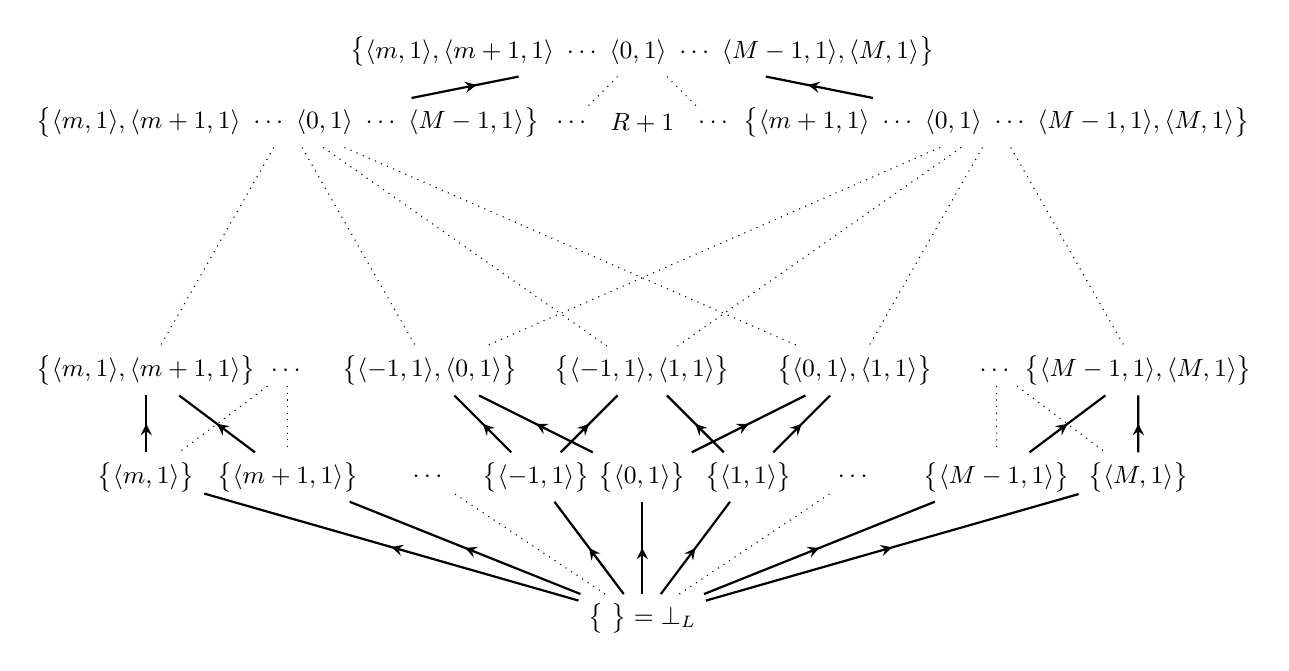
\begin{tikzpicture}[scale=0.45, every node/.style={font=\small}]
\newcommand\XRoot{10}
\newcommand\YRoot{10}
\node (Atop) at (\XRoot,\YRoot) {$\big\{\langle m,1\rangle,\langle m+1,1\rangle\ \cdots\ \langle 0,1\rangle\ \cdots\ \langle M-1,1\rangle,\langle M,1\rangle\big\}$};
\node (A11) at (\XRoot-10,\YRoot-2) {$\big\{\langle m,1\rangle,\langle m+1,1\rangle\ \cdots\ \langle 0,1\rangle\ \cdots\ \langle M-1,1\rangle\big\}$};
\node (A12) at (\XRoot-2,\YRoot-2) {$\qquad\cdots\qquad$};
\node (A13) at (\XRoot,\YRoot-2) {$R+1$};
\node (A14) at (\XRoot+2,\YRoot-2) {$\qquad\cdots\qquad$};
\node (A15) at (\XRoot+10,\YRoot-2) {$\big\{\langle m+1,1\rangle\ \cdots\ \langle 0,1\rangle\ \cdots\ \langle M-1,1\rangle,\langle M,1\rangle\big\}$};
\node (A41) at (\XRoot-14,\YRoot-9) {$\big\{\langle m,1\rangle,\langle m+1,1\rangle\big\}$};
\node (A42) at (\XRoot-10,\YRoot-9) {$\cdots$};
\node (A43) at (\XRoot-6,\YRoot-9) {$\big\{\langle -1,1\rangle,\langle 0,1\rangle\big\}$};
\node (A44) at (\XRoot,\YRoot-9) {$\big\{\langle -1,1\rangle,\langle 1,1\rangle\big\}$};
\node (A45) at (\XRoot+6,\YRoot-9) {$\big\{\langle 0,1\rangle,\langle 1,1\rangle\big\}$};
\node (A46) at (\XRoot+10,\YRoot-9) {$\cdots$};
\node (A47) at (\XRoot+14,\YRoot-9) {$\big\{\langle M-1,1\rangle,\langle M,1\rangle\big\}$};
\node (A51) at (\XRoot-14,\YRoot-12) {$\big\{\langle m,1\rangle\big\}$};
\node (A52) at (\XRoot-10,\YRoot-12) {$\big\{\langle m+1,1\rangle\big\}$};
\node (A53) at (\XRoot-6,\YRoot-12) {$\cdots$};
\node (A54) at (\XRoot-3,\YRoot-12) {$\big\{\langle -1,1\rangle\big\}$};
\node (A55) at (\XRoot,\YRoot-12) {$\big\{\langle 0,1\rangle\big\}$};
\node (A56) at (\XRoot+3,\YRoot-12) {$\big\{\langle 1,1\rangle\big\}$};
\node (A57) at (\XRoot+6,\YRoot-12) {$\cdots$};
\node (A58) at (\XRoot+10,\YRoot-12) {$\big\{\langle M-1,1\rangle\big\}$};
\node (A59) at (\XRoot+14,\YRoot-12) {$\big\{\langle M,1\rangle\big\}$};
\node (Abot) at (\XRoot,\YRoot-16) {$\big\{\ \big\}=\bot_L$};

\path (Atop) edge[-<-] (A11)
			 edge[-<-] (A15)
      (Abot) edge[->-] (A51)
			 edge[->-] (A52)
			 edge[->-] (A54)
			 edge[->-] (A55)
			 edge[->-] (A56)
			 edge[->-] (A58)
			 edge[->-] (A59)
      (A51)  edge[->-] (A41)
      (A52)  edge[->-] (A41)
      (A54)  edge[->-] (A43)
             edge[->-] (A44)
      (A55)  edge[->-] (A43)
             edge[->-] (A45)
      (A56)  edge[->-] (A44)
             edge[->-] (A45)
      (A58)  edge[->-] (A47)
      (A59)  edge[->-] (A47);
      
\path[dotted] (A11)  edge (A41)
                     edge (A43)
                     edge (A44)
                     edge (A45)
              (A15)  edge (A43)
                     edge (A44)
                     edge (A45)
                     edge (A47)
              (Abot) edge (A53)
                     edge (A57)
              (A42)  edge (A51)
                     edge (A52)
              (A46)  edge (A58)
                     edge (A59)
              (Atop) edge (A12)
                     edge (A14);
\end{tikzpicture}

\centerline{\underline{\Large{Frontal View}}}

\begin{tikzpicture}[remember picture, overlay, shift={(32mm, -60mm)}, scale=0.45, every node/.style={font=\small}]
\newcommand\XRoot{10}
\newcommand\YRoot{10}
\node (A01) at (\XRoot-14,\YRoot) {$\big\{\langle m,0\rangle,\langle m+1,1\rangle\ \cdots\ \langle 0,1\rangle\ \cdots\ \langle M-1,1\rangle,\langle M,1\rangle\big\}$};
\node (A02) at (\XRoot-4,\YRoot) {$\qquad\cdots\qquad$};
\node (A03) at (\XRoot,\YRoot) {$R+1$};
\node (A04) at (\XRoot+4,\YRoot) {$\qquad\cdots\qquad$};
\node (A05) at (\XRoot+14,\YRoot) {$\big\{\langle m,1\rangle,\langle m+1,1\rangle\ \cdots\ \langle 0,1\rangle\ \cdots\ \langle M-1,1\rangle,\langle M,0\rangle\big\}$};
\node (A11) at (\XRoot-14,\YRoot-2) {$\big\{\langle m,0\rangle,\langle m+1,1\rangle\ \cdots\ \langle 0,1\rangle\ \cdots\ \langle M-1,1\rangle\big\}$};
\node (A12) at (\XRoot-4,\YRoot-2) {$\qquad\cdots\qquad$};
\node (A13) at (\XRoot,\YRoot-2) {$R+1$};
\node (A14) at (\XRoot+4,\YRoot-2) {$\qquad\cdots\qquad$};
\node (A15) at (\XRoot+14,\YRoot-2) {$\big\{\langle m+1,1\rangle\ \cdots\ \langle 0,1\rangle\ \cdots\ \langle M-1,1\rangle,\langle M,0\rangle\big\}$};
\node (A41) at (\XRoot-18,\YRoot-9) {$\big\{\langle m,0\rangle,\langle A_{\overline{m}},1\rangle\big\}$};
\node (A42) at (\XRoot-12,\YRoot-9) {$\big\{\langle m+1,0\rangle,\langle A_{\overline{m+1}},1\rangle\big\}$};
\node (A43) at (\XRoot-8,\YRoot-9) {$\cdots$};
\node (A44) at (\XRoot-5,\YRoot-9) {$\big\{\langle -1,0\rangle,\langle A_{\overline{-1}},1\rangle\big\}$};
\node (A45) at (\XRoot,\YRoot-9) {$\big\{\langle 0,0\rangle,\langle A_{\overline{0}},1\rangle\big\}$};
\node (A46) at (\XRoot+5,\YRoot-9) {$\big\{\langle 1,0\rangle,\langle A_{\overline{1}},0\rangle\big\}$};
\node (A47) at (\XRoot+8,\YRoot-9) {$\cdots$};
\node (A48) at (\XRoot+12,\YRoot-9) {$\big\{\langle M-1,0\rangle,\langle A_{\overline{M-1}},1\rangle\big\}$};
\node (A49) at (\XRoot+18,\YRoot-9) {$\big\{\langle M,0\rangle,\langle A_{\overline{M}},1\rangle\big\}$};
\node (A51) at (\XRoot-14,\YRoot-12) {$\big\{\langle m,0\rangle\big\}$};
\node (A52) at (\XRoot-10,\YRoot-12) {$\big\{\langle m+1,0\rangle\big\}$};
\node (A53) at (\XRoot-6,\YRoot-12) {$\cdots$};
\node (A54) at (\XRoot-3,\YRoot-12) {$\big\{\langle -1,0\rangle\big\}$};
\node (A55) at (\XRoot,\YRoot-12) {$\big\{\langle 0,0\rangle\big\}$};
\node (A56) at (\XRoot+3,\YRoot-12) {$\big\{\langle 1,0\rangle\big\}$};
\node (A57) at (\XRoot+6,\YRoot-12) {$\cdots$};
\node (A58) at (\XRoot+10,\YRoot-12) {$\big\{\langle M-1,0\rangle\big\}$};
\node (A59) at (\XRoot+14,\YRoot-12) {$\big\{\langle M,0\rangle\big\}$};

\path (A01) edge[-<-=0.8] (A11)
	  (A05) edge[-<-=0.8] (A15)
      (A51) edge[->-] (A41)
      (A52) edge[->-] (A42)
      (A54) edge[->-] (A44)
      (A55) edge[->-] (A45)
      (A56) edge[->-] (A46)
      (A58) edge[->-] (A48)
      (A59) edge[->-] (A49);
      
\path[dotted] (A11)  edge (A41)
              (A15)  edge (A49)
              (A02)  edge (A12)
              (A04)  edge (A14);
\end{tikzpicture}
\\\\\\\\\\\\\\\\\\\\\\\\\\\\
\centerline{\underline{\Large{Frontal View (Cross Sectional)}}}
\\\\
Here, Each element has exactly one tuple with 0 probability and $A_{\overline{p}}\in\{m,m+1\ \cdots\ M-1,M\}\ \setminus\ \{p\}\qquad\forall p\in[m,M]$

\newpage
\begin{tikzpicture}[scale=0.85, every node/.style={font=\small}]
\newcommand\XRoot{-4}
\newcommand\YRoot{20}
\node (A11) at (\XRoot,\YRoot) {$\big\{\langle m,1\rangle,\langle m+1,1\rangle\ \cdots\ \langle 0,1\rangle\ \cdots\ \langle M-1,1\rangle,\langle M,1\rangle\big\}$};
\node (A12) at (\XRoot+13,\YRoot) {$\big\{\langle m,0\rangle,\langle m+1,0\rangle\ \cdots\ \langle 0,0\rangle\ \cdots\ \langle M-1,0\rangle,\langle M,0\rangle\big\}=\top_L$};
\node (A21) at (\XRoot,\YRoot-4) {$\big\{\langle a_1,1\rangle,\langle a_2,1\rangle,\langle a_3,1\rangle\big\}$};
\node (A22) at (\XRoot+4,\YRoot-4) {$\big\{\langle a_1,0\rangle,\langle a_2,1\rangle,\langle a_3,1\rangle\big\}$};
\node (A23) at (\XRoot+8,\YRoot-4) {$\big\{\langle a_1,0\rangle,\langle a_2,0\rangle,\langle a_3,1\rangle\big\}$};
\node (A24) at (\XRoot+12,\YRoot-4) {$\big\{\langle a_1,0\rangle,\langle a_2,0\rangle,\langle a_3,0\rangle\big\}$};
\node (A31) at (\XRoot,\YRoot-6) {$\big\{\langle a_1,1\rangle,\langle a_2,1\rangle\big\}$};
\node (A32) at (\XRoot+4,\YRoot-6) {$\big\{\langle a_1,0\rangle,\langle a_2,1\rangle\big\}$};
\node (A33) at (\XRoot+8,\YRoot-6) {$\big\{\langle a_1,0\rangle,\langle a_2,0\rangle\big\}$};
\node (A41) at (\XRoot,\YRoot-8) {$\big\{\langle a_1,1\rangle\big\}$};
\node (A42) at (\XRoot+4,\YRoot-8) {$\big\{\langle a_1,0\rangle\big\}$};
\node (A51) at (\XRoot,\YRoot-10) {$\big\{\ \big\}=\bot_L$};

\path (A51) edge[->-] (A41)
	  (A41) edge[->-] (A31)
      (A31) edge[->-] (A21)
      (A42) edge[->-] (A32)
      (A32) edge[->-] (A22)
      (A33) edge[->-] (A23);
      
\path[dashed] (A41) edge[->-] (A42)
	          (A32) edge[-<-] (A31)
	          (A32) edge[->-] (A33)
              (A22) edge[-<-=0.0] (A21)
              (A22) edge[->-=1.0] (A23)
              (A23) edge[->-=1.0] (A24);
              
\path[dotted] (A11) edge[->-] (A12)
              (A21) edge[->-] (A11)
	          (A24) edge[->-] (A12);      
\end{tikzpicture}

\centerline{\underline{\Large{Lateral View (Cross Sectional)}}}

Here,
\begin{itemize}
  \item $\bot_L=\big\{\ \big\}\qquad\top_L=\big\{\langle m,0\rangle,\langle m+1,0\rangle\ \cdots\ \langle 0,0\rangle\ \cdots\ \langle M-1,0\rangle,\langle M,0\rangle\big\}$
  \item $a_1,a_2$ and $a_3$ are placeholders with $a_1,a_2,a_3\in[m,M]$
\end{itemize}















\section{\\Proof of $\sqsubseteq_M$ being a partial order}
\label{app:interval_partial}

We prove that $\sqsubseteq_M$ is a partial order relation as follows.

\begin{description}
\item[Reflexivity :] \hfill \\
	It's trivial to show that $\langle[a,b],p_{ab}\rangle\sqsubseteq_M\langle[a,b],p_{ab}\rangle$. It follows directly from our definition of $\sqsubseteq_M$.
\item[Transitivity :] \hfill \\
	$\langle[a,b],p_{ab}\rangle\sqsubseteq_M\langle[c,d],p_{cd}\rangle\qquad\qquad\mathrm{and}\qquad\qquad\langle[c,d],p_{cd}\rangle\sqsubseteq_M\langle[e,f],p_{ef}\rangle\qquad\qquad$ (Given)	
\begin{alignat}{2}
    [a,b]\sqsubseteq_{int}[c,d] &\qquad\land\qquad[c,d]\sqsubseteq_{int}[e,f]\label{eq:po1}\\
	p.m.f\Big(\langle[a,b],p_{ab}\rangle\Big)\geq\ p.m.f\Big(\langle[c,d],p_{cd}\rangle\Big) &\qquad\land\qquad p.m.f\Big(\langle[c,d],p_{cd}\rangle\Big)\geq\ p.m.f\Big(\langle[e,f],p_{ef}\rangle\Big)\label{eq:po2}
\end{alignat}
	
	From \ref{eq:po1} we get $[a,b]\sqsubseteq_{int}[e,f]$ and from \ref{eq:po2} we get $p.m.f\Big(\langle[a,b],p_{ab}\rangle\Big)\geq\ p.m.f\Big(\langle[e,f],p_{ef}\rangle\Big)$.
	
	$\therefore\langle[a,b],p_{ab}\rangle\sqsubseteq_M\langle[e,f],p_{ef}\rangle$
\item[Anti-Symmetricity :] \hfill \\
	$\langle[a,b],p_{ab}\rangle\sqsubseteq_M\langle[c,d],p_{cd}\rangle\qquad\qquad\mathrm{and}\qquad\qquad\langle[c,d],p_{cd}\rangle\sqsubseteq_M\langle[a,b],p_{ab}\rangle\qquad\qquad$ (Given)
\begin{alignat}{2}
    [a,b]\sqsubseteq_{int}[c,d]\implies (c\leq a)\land (b\leq d)&\qquad\qquad\Big[\mathrm{using\ definition}\ \ref{eq:interval_def}\Big]\label{eq:po3}\\
	[c,d]\sqsubseteq_{int}[a,b]\implies (a\leq c)\land (d\leq b)&\qquad\qquad\Big[\mathrm{using\ definition}\ \ref{eq:interval_def}\Big]\label{eq:po4}\\
	p.m.f\Big(\langle[a,b],p_{ab}\rangle\Big)\geq p.m.f\Big(\langle[c,d],p_{cd}\rangle\Big)&\label{eq:po5}\\
	p.m.f\Big(\langle[c,d],p_{cd}\rangle\Big)\geq p.m.f\Big(\langle[a,b],p_{ab}\rangle\Big)&\label{eq:po6}
\end{alignat}

Combining \ref{eq:po3} and \ref{eq:po4} we get,\\
	$(c\leq a)\land (a\leq c)\implies a=c$ and\\
	$(b\leq d)\land (d\leq b)\implies b=d$\\
	$\therefore \underline{a=c,\ b=d}$
	
From \ref{eq:po5} and \ref{eq:po6} we get,\\
	$p.m.f\Big(\langle[a,b],p_{ab}\rangle\Big)=p.m.f\Big(\langle[c,d],p_{cd}\rangle\Big)$\\
	$\Rightarrow \displaystyle\frac{p_{ab}}{b-a+1}=\frac{p_{cd}}{d-c+1}\qquad\qquad\Big[\mathrm{using\ definition}\ \ref{eq:pmf}\Big]$\\
	$\Rightarrow \underline{p_{ab}=p_{cd}}\qquad\qquad\qquad\qquad\Big[\because a=c,\ b=d\quad\mathrm{and}\quad b-a+1\neq0\Big]$
	
	$\therefore\langle[a,b],p_{ab}\rangle=\langle[c,d],p_{cd}\rangle$
\end{description}









\section{\\Proof of correctness of the $l.u.b \displaystyle\bigsqcup_M$ and $g.l.b \displaystyle\bigsqcap^M$ operators in $M$}
\label{app:interval_ub}

\usetikzlibrary{arrows}
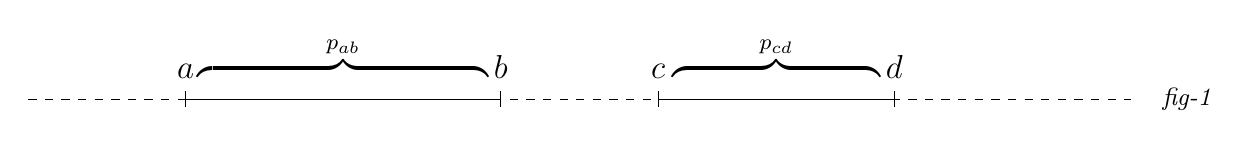
\begin{tikzpicture}[font=\large]
\draw [dashed] (0,0) -- (14,0);
\foreach \x in {2,6,8,11}
\draw [shift={(\x,0)},color=black] (0,3pt) -- (0,-3pt);
\draw (2,0) -- (6,0);
\draw (8,0) -- (11,0);
\draw (2,0) node[above=4pt]{$a$};
\draw (6,0) node[above=4pt]{$b$};
\draw (8,0) node[above=4pt]{$c$};
\draw (11,0) node[above=4pt]{$d$};
\draw (4,0) node[above=4pt]{$\overbrace{\hspace{105pt}}^{p_{ab}}$};
\draw (9.5,0) node[above=4pt]{$\overbrace{\hspace{75pt}}^{p_{cd}}$};
\draw (14,0) node[right=8pt]{\small{\textit{fig-1}}};
\end{tikzpicture}

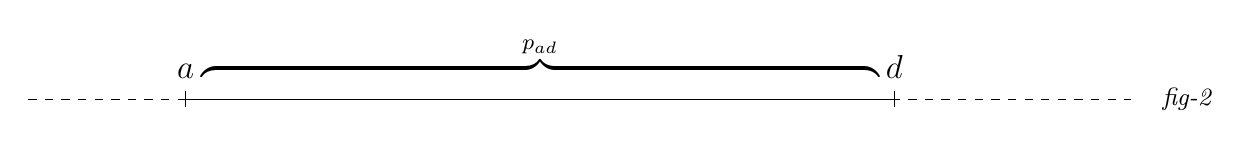
\begin{tikzpicture}[font=\large]
\draw [dashed] (0,0) -- (14,0);
\foreach \x in {2,11}
\draw [shift={(\x,0)},color=black] (0,3pt) -- (0,-3pt);
\draw (2,0) -- (11,0);
\draw (2,0) node[above=4pt]{$a$};
\draw (11,0) node[above=4pt]{$d$};
\draw (6.5,0) node[above=4pt]{$\overbrace{\hspace{245pt}}^{p_{ad}}$};
\draw (14,0) node[right=8pt]{\small{\textit{fig-2}}};
\end{tikzpicture}

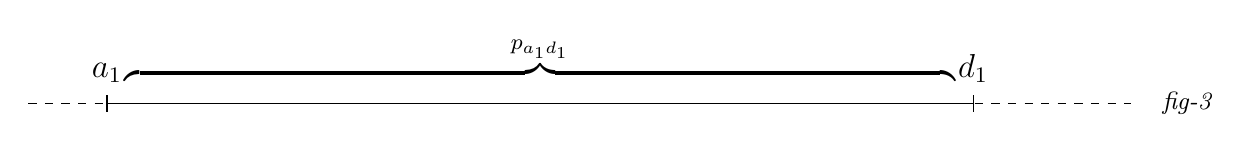
\begin{tikzpicture}[font=\large]
\draw [dashed] (0,0) -- (14,0);
\foreach \x in {1,12}
\draw [shift={(\x,0)},color=black] (0,3pt) -- (0,-3pt);
\draw (1,0) -- (12,0);
\draw (1,0) node[above=4pt]{$a_1$};
\draw (12,0) node[above=4pt]{$d_1$};
\draw (6.5,0) node[above=4pt]{$\overbrace{\hspace{300pt}}^{p_{a_1d_1}}$};
\draw (14,0) node[right=8pt]{\small{\textit{fig-3}}};
\end{tikzpicture}

For the two elements $\langle[a,b],p_{ab}\rangle$ and $\langle[c,d],p_{cd}\rangle$ (in \small{\textit{fig-B1}}) suppose the $l.u.b$ is $\langle[x,y],p_{xy}\rangle$, i.e\\
\centerline{
  $\displaystyle\langle[a,b],p_{ab}\rangle\ \bigsqcup_M\ \langle[c,d],p_{cd}\rangle=\langle[x,y],p_{xy}\rangle$
}
From definition \ref{eq:lub_M} we get,\\
\centerline{
  $x=\mathbf{min}(a,c)=a\qquad y=\mathbf{max}(b,d)=d\qquad\displaystyle p_{xy}=(d-a+1)\ \cdot\ \mathbf{min}\left(p.m.f\Big(\big<[a,\ b],\ p_{ab}\big>\Big),\ p.m.f\Big(\big<[c,\ d],\ p_{cd}\big>\Big),\ \frac{1}{d-a+1}\right)$
}

$\therefore\langle[a,d],p_{ad}\rangle$ (in \small{\textit{fig-2}}) is the $l.u.b$ of the elements in \small{\textit{fig-1}} with $p_{ad}=p_{xy}$. We show all upper bounds of $\langle[a,b],p_{ab}\rangle$ and $\langle[c,d],p_{cd}\rangle$ come higher in the order than $\langle[a,d],p_{ad}\rangle$.

It's trivial to show that for any tuple of the form $\langle[a,d],p'_{ad}\rangle$, where $p'_{ad}\leq p_{ad}\footnote{If $p'_{ad}>p_{ad}$, then $\langle[a,d],p'_{ad}\rangle$ is \textbf{NOT} an upper bound of both $\langle[a,b],p_{ab}\rangle$ and $\langle[c,d],p_{cd}\rangle$}$, $\langle[a,d],p_{ad}\rangle\sqsubseteq_M\langle[a,d],p'_{ad}\rangle$ (by the definition of $\sqsubseteq_M$). So, $\langle[a,d],p_{ad}\rangle$ remains the $l.u.b$.

Now, the other form of tuple i.e $\langle[a_1,d_1],p_{a_1d_1}\rangle$ (in \small{\textit{fig-3}}), where $[a,d]\sqsubseteq_{int}[a_1,d_1]$, will be an upper bound of $\langle[a,b],p_{ab}\rangle$ and $\langle[c,d],p_{cd}\rangle$ if\\
$\langle[a,b],p_{ab}\rangle\sqsubseteq_M\langle[a_1,d_1],p_{a_1d_1}\rangle\qquad\bigwedge\qquad\langle[c,d],p_{cd}\rangle\sqsubseteq_M\langle[a_1,d_1],p_{a_1d_1}\rangle$\\
$\Rightarrow p.m.f\Big(\langle[a_1,d_1],p_{a_1d_1}\rangle\Big)\leq p.m.f\Big(\langle[a,b],p_{ab}\rangle\Big)\ \bigwedge\ p.m.f\Big(\langle[a_1,d_1],p_{a_1d_1}\rangle\Big)\leq p.m.f\Big(\langle[c,d],p_{cd}\rangle\Big)\ \Big[\because \text{we\ know\ }[a,d]\sqsubseteq_{int}[a_1,d_1]\Big]$\\
$\Rightarrow p_{a_1d_1}\leq(d_1-a_1+1)\cdot p.m.f\Big(\langle[a,b],p_{ab}\rangle\Big)\ \bigwedge\ p_{a_1d_1}\leq(d_1-a_1+1)\cdot p.m.f\Big(\langle[c,d],p_{cd}\rangle\Big)\qquad\Big[\text{using\ definition\ }\ref{eq:pmf}\Big]$\\
$\Rightarrow p_{a_1d_1}\leq\mathbf{min}\left((d_1-a_1+1)\cdot p.m.f\Big(\langle[a,b],p_{ab}\rangle\Big),\ (d_1-a_1+1)\cdot p.m.f\Big(\langle[c,d],p_{cd}\rangle\Big),\ 1\right)\qquad\qquad\Big[\because p_{a_1d_1}\leq1\Big]$\\
$\Rightarrow\displaystyle p_{a_1d_1}\leq(d_1-a_1+1)\ \cdot\ \mathbf{min}\left(p.m.f\Big(\big<[a,\ b],\ p_{ab}\big>\Big),\ p.m.f\Big(\big<[c,\ d],\ p_{cd}\big>\Big),\ \frac{1}{d_1-a_1+1}\right)$

We need to prove that, $p.m.f\Big(\big<[a,\ d],\ p_{ad}\big>\Big)\geq p.m.f\Big(\big<[a_1,\ d_1],\ p_{a_1d_1}\big>\Big)$, in order to prove that $\big<[a,\ d],\ p_{ad}\big>$ still remains the $l.u.b$.

Without any loss of generality we assume that
\begin{alignat}{2}
p.m.f\Big(\langle[a,b],p_{ab}\rangle\Big)\leq p.m.f\Big(\langle[c,d],p_{cd}\rangle\Big)\label{eq:ub1}\\
\frac{1}{d_1-a_1+1}<\frac{1}{d-a+1}\label{eq:ub2}
\end{alignat}
\begin{equation*}
 \left.\begin{aligned}
        p_{ad}&=(d-a+1)\ \cdot\ \mathbf{min}\left(p.m.f\Big(\langle[a,b],p_{ab}\rangle\Big),\ p.m.f\Big(\langle[c,d],p_{cd}\rangle\Big),\ \frac{1}{d-a+1}\right)\\
        &=(d-a+1)\ \cdot\ \mathbf{min}\left(p.m.f\Big(\langle[a,b],p_{ab}\rangle\Big),\ \frac{1}{d-a+1}\right)\qquad[\mathrm{from}\ \ref{eq:ub1}]\\
        p_{a_1d_1}&=(d_1-a_1+1)\ \cdot\ \mathbf{min}\left(p.m.f\Big(\langle[a,b],p_{ab}\rangle\Big),\ p.m.f\Big(\langle[c,d],p_{cd}\rangle\Big),\ \frac{1}{d_1-a_1+1}\right)\\
        &=(d_1-a_1+1)\ \cdot\ \mathbf{min}\left(p.m.f\Big(\langle[a,b],p_{ab}\rangle\Big),\ \frac{1}{d_1-a_1+1}\right)\qquad[\mathrm{from}\ \ref{eq:ub1}]
       \end{aligned}\qquad
 \right\}
 \qquad \text{(Given)}
\end{equation*}

In view of \ref{eq:ub2} there are three cases to consider now.

\begin{description}
	\item[Case 1 : $\qquad\displaystyle p.m.f\Big(\langle\lbrack a,b\rbrack,p_{ab}\rangle\Big)\leq\frac{1}{d_1-a_1+1}$] \hfill
	$$\therefore \displaystyle p.m.f\Big(\langle[a,b],p_{ab}\rangle\Big)<\frac{1}{d-a+1}\qquad[\mathrm{from}\ \ref{eq:ub2}]$$
	$$\therefore p_{ad}=(d-a+1)\ \cdot\ p.m.f\Big(\langle[a,b],p_{ab}\rangle\Big)\qquad p_{a_1d_1}=(d_1-a_1+1)\ \cdot\ p.m.f\Big(\langle[a,b],p_{ab}\rangle\Big)$$
	$$\therefore p.m.f\Big(\langle[a,d],p_{ad}\rangle\Big)=p.m.f\Big(\langle[a_1,d_1],p_{a_1d_1}\rangle\Big)$$
	\item[Case 2 : $\qquad\displaystyle \frac{1}{d_1-a_1+1}<p.m.f\Big(\langle\lbrack a,b\rbrack,p_{ab}\rangle\Big)<\frac{1}{d-a+1}$] \hfill
	$$\therefore p_{ad}=(d-a+1)\ \cdot\ p.m.f\Big(\langle[a,b],p_{ab}\rangle\Big)\qquad p_{a_1d_1}=1$$
	$$\therefore p.m.f\Big(\langle[a,d],p_{ad}\rangle\Big)=p.m.f\Big(\langle[a,b],p_{ab}\rangle\Big)\qquad p.m.f\Big(\langle[a_1,d_1],p_{a_1d_1}\rangle\Big)=\frac{1}{d_1-a_1+1}$$
	$$\therefore p.m.f\Big(\langle[a,d],p_{ad}\rangle\Big)>p.m.f\Big(\langle[a_1,d_1],p_{a_1d_1}\rangle\Big)$$
	\item[Case 3 : $\qquad\displaystyle \frac{1}{d-a+1}\leq p.m.f\Big(\langle\lbrack a,b\rbrack,p_{ab}\rangle\Big)$] \hfill
	$$\therefore \displaystyle p.m.f\Big(\langle[a,b],p_{ab}\rangle\Big)>\frac{1}{d_1-a_1+1}\qquad[\mathrm{from}\ \ref{eq:ub2}]$$
	$$\therefore p_{ad}=1\qquad p_{a_1d_1}=1$$
	$$\therefore p.m.f\Big(\langle[a,d],p_{ad}\rangle\Big)=\ p.m.f\Big(\langle[a_1,d_1],p_{a_1d_1}\rangle\Big)$$
\end{description}

In all the above three cases $p.m.f\Big(\langle[a,d],p_{ad}\rangle\Big)\geq p.m.f\Big(\langle[a_1,d_1],p_{a_1d_1}\rangle\Big)$. Hence $\langle[a,d],p_{ad}\rangle$ is the $l.u.b$

Analogous arguments can be applied to show the soundness of the greatest lower bound, $\displaystyle\bigsqcap^M$ definition. For brevity we're omitting the proof for $g.l.b$ here.









\newpage
\section{\\Hasse Diagram of the Probabilistic Interval Lattice $(M,\sqsubseteq_M)$}
\label{app:interval_hasse}

The lattice $(M,\sqsubseteq_M)$ is best viewed in 3 dimensions. For that reason we've given 4 different views of the same lattice.

In all the following diagrams, \underline{\textbf{solid lines}} represent direct parent-child relationship i.e there doesn't exist any other element between the connecting nodes and \underline{\textbf{dashed lines}} represent the existence of infinite number of elements having same intervals as that of the connecting nodes but probability that varies monotonically between the connecting nodes.\\

\centerline{
  \psset{arrowscale=1.5, ArrowInside=-<}
  \pstree[levelsep=40pt, nodesep=4pt]{\Tr{$\top_M=\big<[m,M],0\big>$}}{
    \pstree{\Tr[name=L2C1]{$\big<[m,M-1],0\big>$}}{
      \psset{ArrowInside=-}
      \pstree{\psset{linestyle=none}\Tr{}}{
        \pstree{\psset{linestyle=none}\Tr{}}{
          \pstree{\psset{linestyle=none}\Tr{}}{
            \pstree{\psset{linestyle=none}\Tr[name=L6C1]{$\big<[m,M-2],0\big>$}}{
              \psset{linestyle=dotted}
              \pstree{\Tr[name=L7C1]{$\big<[m,m],0\big>$}}{
                \psset{linestyle=dashed, ArrowInside=-<}
                \Tr[name=L8C1]{$\big<[m,m],\epsilon\big>$}
              }
            }
          }
        }
      }
    }
    \pstree{\psset{linestyle=dashed}\Tr[name=L2C2]{$\big<[m,M],\epsilon\big>$}}{
      \pstree{\Tr[name=L3C1]{$\big<[m,M-1],\frac{\epsilon\cdot(M-m)}{M-m+1}\big>$}}{
        \psset{linestyle=dashed}
        \Tr[name=L4C1]{$\big<[m,M-1],\epsilon_2\big>$}
        \psset{linestyle=none,ArrowInside=-}
        \Tr{$\qquad\qquad$}
        \Tr{$\qquad\qquad\qquad$}
      }
      \pstree{\psset{linestyle=dashed}\Tr[name=L3C2]{$\big<[m,M],\epsilon_1\big>$}}{
        \pstree{\psset{linestyle=dashed}\Tr[name=L4C2]{$\big<[m,M],1\big>$}}{
          \pstree{\Tr[name=L5C1]{$\big<[m,M-1],\frac{M-m}{M-m+1}\big>$}}{
            \psset{linestyle=dashed}
            \pstree{\Tr[name=L6C2]{$\big<[m,M-1],1\big>$}}{
              \psset{linestyle=solid}
              \pstree{\Tr[name=L7C2]{$\big<[m,M-2],\frac{M-m-1}{M-m}\big>$}}{
                \psset{linestyle=dashed,ArrowInside=-<}
                \pstree{\Tr[name=L8C2]{$\big<[m,M-2],1\big>$}}{
                  \psset{linestyle=dotted,ArrowInside=-}
                  \Tr[name=L9C1]{$\big<[m,m],1\big>$}
                }
              }
            }
          }
          \psset{linestyle=none}
          \pstree{\psset{ArrowInside=-}\Tr{}}{
            \pstree{\psset{ArrowInside=-}\Tr[name=L6C3]{$\big<[m+1,M-1],0\big>$}}{
              \psset{linestyle=dashed}
              \pstree{\Tr[name=L7C3]{$\big<[m+1,M-1],\frac{M-m-1}{M-m}\big>$}}{
                \pstree{\Tr[name=L8C3]{$\big<[m+1,M-1],1\big>$}}{
                  \psset{linestyle=dotted,ArrowInside=-}
                  \Tr[name=L9C2]{$\big<[m+1,m+1],1\big>$}
                  \psset{linestyle=none}
                  \pstree{\Tr[name=L9C3]{$\ldots\quad\big<[0,0],1\big>\quad\ldots$}}{
                    \psset{linestyle=solid,ArrowInside=-<}
                    \pstree{\Tr[name=L10C1]{$\bot_M=\big<[\ ],1\big>$}}{
                    }
                  }
                  \psset{linestyle=dotted}
                  \Tr[name=L9C4]{$\big<[M-1,M-1],1\big>$}
                }
              }
            }
          }
          \psset{linestyle=solid}
          \pstree{\Tr[name=L5C2]{$\big<[m+1,M],\frac{M-m}{M-m+1}\big>$}}{
            \psset{linestyle=dashed}
            \pstree{\Tr[name=L6C4]{$\big<[m+1,M],1\big>$}}{
              \psset{linestyle=solid}
              \pstree{\Tr[name=L7C4]{$\big<[m+2,M],\frac{M-m-1}{M-m}\big>$}}{
                \psset{linestyle=dashed,ArrowInside=-<}
                \pstree{\Tr[name=L8C4]{$\big<[m+2,M],1\big>$}}{
                  \psset{linestyle=dotted,ArrowInside=-}
                  \Tr[name=L9C5]{$\big<[M,M],1\big>$}
                }
              }
            }
          }
        }
      }
      \psset{linestyle=solid}
      \pstree{\Tr[name=L3C3]{$\big<[m+1,M],\frac{\epsilon\cdot(M-m)}{M-m+1}\big>$}}{
        \psset{linestyle=none,ArrowInside=-}
        \Tr{$\qquad\qquad$}
        \Tr{$\qquad\qquad\qquad$}
        \psset{linestyle=dashed,ArrowInside=-<}
        \Tr[name=L4C3]{$\big<[m+1,M],\epsilon_2\big>$}
      }
    }
    \pstree{\Tr[name=L2C3]{$\big<[m+1,M],0\big>$}}{
      \psset{ArrowInside=-}
      \pstree{\psset{linestyle=none}\Tr{}}{
        \pstree{\psset{linestyle=none}\Tr{}}{
          \pstree{\psset{linestyle=none}\Tr{}}{
            \pstree{\psset{linestyle=none}\Tr[name=L6C5]{$\big<[m+2,M],0\big>$}}{
              \psset{linestyle=dotted}
              \pstree{\Tr[name=L7C5]{$\big<[M,M],0\big>$}}{
                \psset{linestyle=dashed,ArrowInside=-<}
                \Tr[name=L8C5]{$\big<[M,M],\epsilon\big>$}
              }
            }
          }
        }
      }
    }
  }
  \psset{nodesep=4pt}
  \ncline{L2C1}{L6C1}
  \ncline{L2C3}{L6C5}
  \ncline{L2C1}{L6C3}
  \ncline{L2C3}{L6C3}
  \ncline{L3C2}{L4C1}
  \ncline{L3C2}{L4C3}
  \ncline{L6C2}{L7C3}
  \ncline{L6C4}{L7C3}
  \ncline{L9C1}{L10C1}
  \ncline{L9C2}{L10C1}
  \ncline{L9C4}{L10C1}
  \ncline{L9C5}{L10C1}
  \ncline[linestyle=dashed]{L2C1}{L3C1}
  \ncline[linestyle=dashed]{L2C3}{L3C3}
  \ncline[linestyle=dashed]{L4C1}{L5C1}
  \ncline[linestyle=dashed]{L4C3}{L5C2}
  \ncline[linestyle=dashed]{L8C1}{L9C1}
  \ncline[linestyle=dashed]{L8C5}{L9C5}
  \ncline[linestyle=dashed]{L6C1}{L7C2}
  \ncline[linestyle=dashed]{L6C5}{L7C4}
}
\centerline{\underline{\Large{2D Projectional View}}}
\hfill\\

\hfill*legends are defined in the next page

\newpage
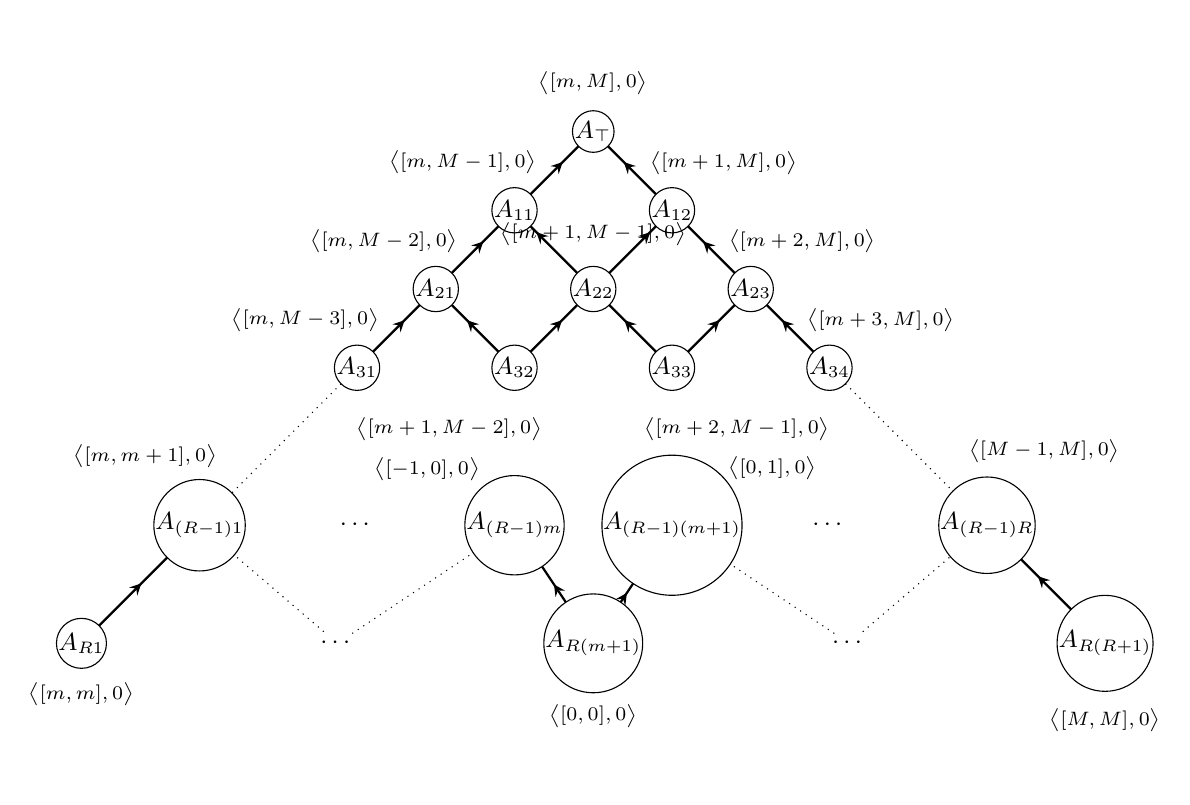
\begin{tikzpicture}[scale=0.5, every node/.style={draw, circle, inner sep=0pt, outer sep=0pt, font=\small}]
\newcommand\XRoot{12}
\newcommand\YRoot{12}
\node[label={[label distance=-10pt, font=\scriptsize]90:$\big<[m,M],0\big>$}] (Atop) at (\XRoot,\YRoot) {$A_\top$};
\node[label={[label distance=-10pt, font=\scriptsize]100:$\big<[m,M-1],0\big>$}] (A11) at (\XRoot-2,\YRoot-2) {$A_{11}$};
\node[label={[label distance=-10pt, font=\scriptsize]80:$\big<[m+1,M],0\big>$}] (A12) at (\XRoot+2,\YRoot-2) {$A_{12}$};
\node[label={[label distance=-10pt, font=\scriptsize]100:$\big<[m,M-2],0\big>$}] (A21) at (\XRoot-4,\YRoot-4) {$A_{21}$};
\node[label={[label distance=-22pt, font=\scriptsize]above:$\big<[m+1,M-1],0\big>$}] (A22) at (\XRoot,\YRoot-4) {$A_{22}$};
\node[label={[label distance=-10pt, font=\scriptsize]80:$\big<[m+2,M],0\big>$}] (A23) at (\XRoot+4,\YRoot-4) {$A_{23}$};
\node[label={[label distance=-10pt, font=\scriptsize]100:$\big<[m,M-3],0\big>$}] (A31) at (\XRoot-6,\YRoot-6) {$A_{31}$};
\node[label={[label distance=-10pt, font=\scriptsize]-100:$\big<[m+1,M-2],0\big>$}] (A32) at (\XRoot-2,\YRoot-6) {$A_{32}$};
\node[label={[label distance=-10pt, font=\scriptsize]-80:$\big<[m+2,M-1],0\big>$}] (A33) at (\XRoot+2,\YRoot-6) {$A_{33}$};
\node[label={[label distance=-10pt, font=\scriptsize]80:$\big<[m+3,M],0\big>$}] (A34) at (\XRoot+6,\YRoot-6) {$A_{34}$};
\node[label={[label distance=-10pt, font=\scriptsize]100:$\big<[m,m+1],0\big>$}] (All1) at (\XRoot-10,\YRoot-10) {$A_{(R-1)1}$};
\node[draw=none] at (\XRoot-6,\YRoot-10) {$\cdots$};
\node[label={[label distance=1pt, font=\scriptsize]-200:$\big<[-1,0],0\big>$}] (All2) at (\XRoot-2,\YRoot-10) {$A_{(R-1)m}$};
\node[label={[label distance=1pt, font=\scriptsize]20:$\big<[0,1],0\big>$}] (All3) at (\XRoot+2,\YRoot-10) {$A_{(R-1)(m+1)}$};
\node[draw=none] at (\XRoot+6,\YRoot-10) {$\cdots$};
\node[label={[label distance=-10pt, font=\scriptsize]80:$\big<[M-1,M],0\big>$}] (All4) at (\XRoot+10,\YRoot-10) {$A_{(R-1)R}$};
\node[label={[label distance=-10pt, font=\scriptsize]-90:$\big<[m,m],0\big>$}] (Al1) at (\XRoot-13,\YRoot-13) {$A_{R1}$};
\node[draw=none] (Al2) at (\XRoot-6.5,\YRoot-13) {$\cdots$};
\node[label={[label distance=-8pt, font=\scriptsize]-90:$\big<[0,0],0\big>$}] (Al3) at (\XRoot,\YRoot-13) {$A_{R(m+1)}$};
\node[draw=none] (Al4) at (\XRoot+6.5,\YRoot-13) {$\cdots$};
\node[label={[label distance=-10pt, font=\scriptsize]-90:$\big<[M,M],0\big>$}] (Al5) at (\XRoot+13,\YRoot-13) {$A_{R(R+1)}$};

\path (Atop) edge[-<-] (A11)
             edge[-<-] (A12)
      (A11)  edge[-<-] (A21)
             edge[-<-=0.3] (A22)
      (A12)  edge[-<-=0.3] (A22)
             edge[-<-] (A23)
      (A21)  edge[-<-] (A31)
             edge[-<-] (A32)
      (A22)  edge[-<-] (A32)
             edge[-<-] (A33)
      (A23)  edge[-<-] (A33)
             edge[-<-] (A34)
      (All1) edge[-<-] (Al1)
      (Al3)  edge[->-] (All2)
             edge[->-] (All3)
      (All4) edge[-<-] (Al5);
      
\path[dotted] (A31) edge (All1)
              (Al2) edge (All1)
                    edge (All2)
              (Al4) edge (All3)
                    edge (All4)
              (A34) edge (All4);
\end{tikzpicture}

\centerline{\underline{\Large{Frontal View}}}

\begin{description}
  \item[In the 2D Projectional View :] \hfill
	\begin{itemize}
	  \item $m=\mathtt{MININT}$
	  \item $M=\mathtt{MAXINT}$
	  \item $0<\epsilon,\epsilon_1,\epsilon_2<1$
	  \item $\epsilon_2=\displaystyle\frac{\epsilon_1\cdot(M-m)}{M-m+1}\quad\footnote{In general probability of an element = $\displaystyle\frac{\mathrm{(Probability\ of\ its\ direct\ parent)}\times\mathrm{(No.\ of\ elements\ in\ its\ own\ interval)}}{\mathrm{(No.\ of\ elements\ in\ its\ direct\ parent's\ interval)}}$}$
	\end{itemize}
  \item[In the Frontal \& Lateral View :] \hfill\\
    $A_{Ri}\equiv A_{(M-m)i}\quad\text{and}\quad\hat{A}_{Ri}\equiv\hat{A}_{(M-m)i}\qquad\forall i$\\
    For every pair of indices $i, j$ (and $\top$) the elements denoted by $A_{ij}$ (and $A_\top$) and $\hat{A}_{ij}$ (and $\hat{A}_\top$) have the same interval, but probability in element $A_{ij}$ (and $A_\top$) is $0$ , wherese it is 1 for $\hat{A}_{ij}$ (and $\hat{A}_\top$).\\
    E.g: $A_{22}\equiv\big<[m+1,\ M-1],\ 0\big>$ but $\hat{A}_{22}\equiv\big<[m+1,\ M-1],\ 1\big>$
\end{description}

\newpage
\begin{tikzpicture}[x={(6mm,-3.5mm)}, y={(0mm,15mm)}, z={(14mm,0mm)}, every node/.style={inner sep=2pt}, scale=0.9, remember picture, overlay, shift={(-20mm, -70mm)}]
\newcommand\Root{8}
\newcommand\Zoffset{8}
\newcommand\InitialBlack{0.7}
\node (A1) at (\Root,\Root,0) {$A_{\top}$};
\node (A2) at (\Root-1,\Root-1,0) {$A_{11}$};
\node (A3) at (\Root+1,\Root-1,0) {$A_{12}$};
\node (A4) at (\Root-2,\Root-2,0) {$A_{21}$};
\node (A5) at (\Root,\Root-2,0) {$A_{22}$};
\node (A6) at (\Root+2,\Root-2,0) {$A_{23}$};
\node (A7) at (\Root-3,\Root-3,0) {$A_{31}$};
\node (A8) at (\Root-1,\Root-3,0) {$A_{32}$};
\node (A9) at (\Root+1,\Root-3,0) {$A_{33}$};
\node (A10) at (\Root+3,\Root-3,0) {$A_{34}$};
\node (All1) at (\Root-5,\Root-5,0) {$A_{(R-1)1}$};
\node at (\Root-3,\Root-5,0) {$\ddots$};
\node (All2) at (\Root-1,\Root-5,0) {$A_{(R-1)m}$};
\node (All3) at (\Root+1,\Root-5,0) {$A_{(R-1)(m+1)}$};
\node at (\Root+3,\Root-5,0) {$\ddots$};
\node (All4) at (\Root+5,\Root-5,0) {$A_{(R-1)R}$};
\node (Al1) at (\Root-6,\Root-6,0) {$A_{R1}$};
\node (Al2) at (\Root-3,\Root-6,0) {$\ddots$};
\node (Al3) at (\Root,\Root-6,0) {$A_{R(m+1)}$};
\node (Al4) at (\Root+3,\Root-6,0) {$\ddots$};
\node (Al5) at (\Root+6,\Root-6,0) {$A_{R(R+1)}$};

\node (B1) at (\Root,\Root,\Zoffset) {$\hat{A}_{\top}$};
\node[lightgray] (B2) at (\Root-1,\Root-1,\Zoffset) {$\hat{A}_{11}$};
\node (B3) at (\Root+1,\Root-1,\Zoffset) {$\hat{A}_{12}$};
\node[lightgray] (B4) at (\Root-2,\Root-2,\Zoffset) {$\hat{A}_{21}$};
\node[inner sep=0pt] (B5) at (\Root,\Root-2,\Zoffset) {$\hat{A}_{22}$};
\node (B6) at (\Root+2,\Root-2,\Zoffset) {$\hat{A}_{23}$};
\node[lightgray] (B7) at (\Root-3,\Root-3,\Zoffset) {$\hat{A}_{31}$};
\node[lightgray] (B8) at (\Root-1,\Root-3,\Zoffset) {$\hat{A}_{32}$};
\node (B9) at (\Root+1,\Root-3,\Zoffset) {$\hat{A}_{33}$};
\node (B10) at (\Root+3,\Root-3,\Zoffset) {$\hat{A}_{34}$};
\node[lightgray] (Bll1) at (\Root-5,\Root-5,\Zoffset) {$\hat{A}_{(R-1)1}$};
\node[lightgray] (Bll2) at (\Root-1,\Root-5,\Zoffset) {$\hat{A}_{(R-1)m}$};
\node (Bll3) at (\Root+1,\Root-5,\Zoffset) {$\hat{A}_{(R-1)(m+1)}$};
\node (Bll4) at (\Root+5,\Root-5,\Zoffset) {$\hat{A}_{(R-1)R}$};
\node[lightgray] (Bl1) at (\Root-6,\Root-6,\Zoffset) {$\hat{A}_{R1}$};
\node[lightgray] (Bl2) at (\Root-3,\Root-6,\Zoffset) {$\ddots$};
\node (Bl3) at (\Root,\Root-6,\Zoffset) {$\hat{A}_{R(m+1)}$};
\node (Bl4) at (\Root+3,\Root-6,\Zoffset) {$\ddots$};
\node (Bl5) at (\Root+6,\Root-6,\Zoffset) {$\hat{A}_{R(R+1)}$};
\node (Bottom) at (\Root,\Root-8,\Zoffset) {$A_{\bot}$};

\path[dashed] (A1)   edge (B1)
              (A3)   edge[-<-=0.97] (B3)
              (A6)   edge[-<-=0.92] (B6)
              (A10)  edge[-<-=0.85] (B10)
              (All4) edge[-<-=0.9] (Bll4)
              (Al5)  edge[-<-=0.9] (Bl5);

\draw[dashed] (A2) -- (\Root-1,\Root-1,\InitialBlack) (A4) -- (\Root-2,\Root-2,\InitialBlack) (A5) -- (\Root,\Root-2,\InitialBlack) (A7) -- (\Root-3,\Root-3,\InitialBlack) (A8) -- (\Root-1,\Root-3,\InitialBlack) (A9) -- (\Root+1,\Root-3,\InitialBlack) (All1) -- (\Root-5,\Root-5,\InitialBlack*5) (All2) -- (\Root-1,\Root-5,\InitialBlack*3) (All3) -- (\Root+1,\Root-5,\InitialBlack*2) (Al1) -- (\Root-6,\Root-6,\InitialBlack*1.2) (Al3) -- (\Root,\Root-6,\InitialBlack*1.2);

\draw[lightgray, dashed] (\Root-1,\Root-1,\InitialBlack) -- (B2) (\Root-2,\Root-2,\InitialBlack) -- (B4) (\Root,\Root-2,\InitialBlack) -- (B5) (\Root-3,\Root-3,\InitialBlack) -- (B7) (\Root-1,\Root-3,\InitialBlack) -- (B8) (\Root+1,\Root-3,\InitialBlack) -- (\Root+1,\Root-3,\Zoffset-0.7) (\Root-5,\Root-5,\InitialBlack*5) -- (Bll1) (\Root-1,\Root-5,\InitialBlack*3) -- (Bll2) (\Root+1,\Root-5,\InitialBlack*2) -- (Bll3) (\Root-6,\Root-6,\InitialBlack*1.2) -- (Bl1) (\Root,\Root-6,\InitialBlack*1.2) -- (\Root,\Root-6,\Zoffset-0.8);

\draw[dashed] (\Root+1,\Root-3,\Zoffset-0.7) -- (B9) (\Root,\Root-6,\Zoffset-0.8) -- (Bl3);

\draw (A1) -- (A2) -- (A4) -- (A7) (A1) -- (A3) -- (A6) -- (A10);

\draw (A2) -- (A5) (A3) -- (A5) (A4) -- (A8) (A5) -- (A8) (A5) -- (A9) (A6) -- (A9) (All1) -- (Al1) (All4) -- (Al5) (All2) -- (Al3) (All3) -- (Al3) (Bl5) -- (Bottom) -- (\Root+6,\Root-5.5,\Zoffset*0.679) (Bottom) -- (\Root+5.75,\Root-5.78,\Zoffset*0.61);

\draw[dotted] (A7) -- (All1) -- (Al2) (A10) -- (All4) -- (Al4) (All2) -- (Al2) (All3) -- (Al4) (B10) -- (\Root+5,\Root-5,\Zoffset*0.6) (Bl2) -- (Bottom) -- (Bl4);

\draw (B1) edge[-<-=0.3] (\Root+1,\Root-1,\Zoffset*0.9) (B3) edge[-<-=0.2] (\Root+2,\Root-2,\Zoffset*0.8) (B6) edge[-<-=0.4] (\Root+3,\Root-3,\Zoffset*0.7) (Bll4) edge[-<-=0.4] (\Root+6,\Root-6,\Zoffset*0.5);

\draw[lightgray] (B1) edge[-<-] (\Root-1,\Root-1,\Zoffset*0.9) (B2) edge[-<-=0.2] (\Root,\Root-2,\Zoffset*0.8) (B2) edge[-<-=0.3] (\Root-2,\Root-2,\Zoffset*0.8) (B3) edge[-<-=0.4] (\Root,\Root-2,\Zoffset*0.8) (B4) edge[-<-=0.4] (\Root-3,\Root-3,\Zoffset*0.7) (B4) edge[-<-] (\Root-1,\Root-3,\Zoffset*0.7) (B5) edge[-<-=0.8] (\Root-1,\Root-3,\Zoffset*0.7) (B5) edge[-<-=0.7] (\Root+1,\Root-3,\Zoffset*0.7) (B6) edge[-<-=0.7] (\Root+1,\Root-3,\Zoffset*0.7) (Bll1) edge[-<-] (\Root-6,\Root-6,\Zoffset*0.5) (Bll2) edge[-<-=0.6] (\Root,\Root-6,\Zoffset*0.5) (Bll3) edge[-<-=0.6] (\Root,\Root-6,\Zoffset*0.5) (Bl3) edge[-<-] (\Root+6,\Root-5.5,\Zoffset*0.679) (\Root+5.75,\Root-5.78,\Zoffset*0.61) -- (Bl1);
\end{tikzpicture}
\\\\\\\\\\\\\\\\\\\\\\\\\\\\\\\\\\\\\\\\\\\\\\\\\\\
\centerline{\underline{\Large{Lateral View (Skewed)}}}
\begin{tikzpicture}[remember picture, overlay, shift={(0mm, -90mm)}]
\newcommand\XRoot{8}
\newcommand\YRoot{8}
\node at (\XRoot,\YRoot) {$\hat{A}_\top$};
\node at (\XRoot-1,\YRoot-1) {$\hat{A}_{12}$};
\node at (\XRoot+1,\YRoot-1) {$\hat{A}_{11}$};
\node at (\XRoot-2,\YRoot-2) {$\hat{A}_{23}$};
\node at (\XRoot,\YRoot-2) {$\hat{A}_{22}$};
\node at (\XRoot+2,\YRoot-2) {$\hat{A}_{21}$};
\node[inner sep=15pt] (A34) at (\XRoot-3,\YRoot-3) {$\hat{A}_{34}$};
\node at (\XRoot-1,\YRoot-3) {$\hat{A}_{33}$};
\node at (\XRoot+1,\YRoot-3) {$\hat{A}_{32}$};
\node[inner sep=15pt] (A31) at (\XRoot+3,\YRoot-3) {$\hat{A}_{31}$};
\node[inner sep=15pt] (All6) at (\XRoot-5,\YRoot-5) {$\hat{A}_{(R-1)R}$};
\node at (\XRoot-3,\YRoot-5) {$\cdots$};
\node at (\XRoot-1,\YRoot-5) {$\hat{A}_{(R-1)(m+1)}$};
\node at (\XRoot+1,\YRoot-5) {$\hat{A}_{(R-1)m}$};
\node at (\XRoot+3,\YRoot-5) {$\cdots$};
\node[inner sep=15pt] (All1) at (\XRoot+5,\YRoot-5) {$\hat{A}_{(R-1)1}$};
\node (L1) at (\XRoot-6,\YRoot-6) {$\hat{A}_{R(R+1)}$};
\node (L2) at (\XRoot-3,\YRoot-6) {$\cdots$};
\node (L3) at (\XRoot,\YRoot-6) {$\hat{A}_{R(m+1)}$};
\node (L4) at (\XRoot+3,\YRoot-6) {$\cdots$};
\node (L5) at (\XRoot+6,\YRoot-6) {$\hat{A}_{R1}$};
\node (Bottom) at (\XRoot,\YRoot-8) {$A_\bot$};

\path (Bottom) edge[->-] (L1)
               edge[->-] (L3)
               edge[->-] (L5);

\draw[dotted] (L2) -- (Bottom) -- (L4) (A34) -- (All6) (A31) -- (All1);
\end{tikzpicture}
\\\\\\\\\\\\\\\\\\\\\\\\\\\\\\\\\\\\\\\\\\\\\\\\\\\\\
\centerline{\underline{\Large{Rear View}}}
\newpage








\section{\\Proof of monotonicity of Galois connection $(\alpha,\gamma)$}
\label{app:monotonicity}

Let, $\langle[a,b],p_{ab}\rangle$ and $\langle[c,d],p_{cd}\rangle$ be two elements in $M$, with $\langle[a,b],p_{ab}\rangle\sqsubseteq_M\langle[c,d],p_{cd}\rangle$. We show that

\centerline{
  $\GAMMA$$\Big(\langle[a,b],p_{ab}\rangle\Big)\sqsubseteq_L\ $$\GAMMA$$\Big(\langle[c,d],p_{cd}\rangle\Big)$\footnote{This is trivial to show that, if $\bot_M\sqsubseteq_M\langle[a,b],p_{ab}\rangle$ then $\GAMMA$$\Big(\bot_M\Big)=\bot_L\sqsubseteq_L\ $$\GAMMA$$\Big(\langle[a,b],p_{ab}\rangle\Big)$ using definition \ref{eq:gamma}}
}

$\because\langle[a,b],p_{ab}\rangle\sqsubseteq_M\langle[c,d],p_{cd}\rangle$, from our definition of $\sqsubseteq_M$ we have
\begin{flalign}
  &[a,b]\sqsubseteq_{int}[c,d]\qquad\qquad\text{and}\nonumber&&\\
  &p.m.f\big(\langle[a,b],p_{ab}\rangle\big)\geq p.m.f\big(\langle[c,d],p_{cd}\rangle\big)\label{eq:monotone1}&&
\end{flalign}
\begin{align}
            &\quad[a,b]\sqsubseteq_{int}[c,d]&\nonumber\\
\Rightarrow &\quad c\leq a\bigwedge b\leq d&[\text{using definition } \ref{eq:interval_def}]\nonumber\\
\Rightarrow &\quad \big\{i\ |\ i\in[a,b]\big\}\subseteq\big\{i\ |\ i\in[c,d]\big\}\label{eq:monotone2}&
\end{align}
$\GAMMA$$\Big(\langle[a,b],p_{ab}\rangle\Big)=\Big\{\big\langle i, p.m.f\big(\langle[a,b],p_{ab}\rangle\big)\big\rangle\quad\big|\quad i\in[a,b]\Big\}=X\text{ (say)}\qquad$ and\\
$\GAMMA$$\Big(\langle[c,d],p_{cd}\rangle\Big)=\Big\{\big\langle i, p.m.f\big(\langle[c,d],p_{cd}\rangle\big)\big\rangle\quad\big|\quad i\in[c,d]\Big\}=Y\text{ (say)}$

\noindent From \ref{eq:monotone2} we get $\quad\big\{\mathbf{val}(t_x)\ |\ t_x\in X\big\}\subseteq\big\{\mathbf{val}(t_y)\ |\ t_y\in Y\big\}\quad$ and\\
from \ref{eq:monotone1} we get $\quad\forall t_x\in X,\forall t_y\in Y\ \bigg(\Big(\mathbf{val}(t_x)=\mathbf{val}(t_y)\Big)\Rightarrow\Big(\mathbf{prob}(t_x)\geq\mathbf{prob}(t_y)\Big)\bigg)$

$\therefore\ X\sqsubseteq_L Y\qquad\qquad[\text{from our definition of } \sqsubseteq_L]$.

$\therefore$$\ \GAMMA$$\Big(\langle[a,b],p_{ab}\rangle\Big)\sqsubseteq_L\ $$\GAMMA$$\Big(\langle[c,d],p_{cd}\rangle\Big)$

\noindent This completes the proof that $\GAMMA$ is monotonic.

\noindent\rule{10cm}{0.1pt}

Now, suppose $A$ and $B$ are two elements in $L$, with $A\sqsubseteq_L B$ and $A,B\neq\{\ \}$. We show that

\centerline{
  $\ALPHA$$\Big(A\Big)\sqsubseteq_M\ $$\ALPHA$$\Big(B\Big)$\footnote{It's a trivial case, if $\bot_L\sqsubseteq_L S, \forall S\in L\quad$ then $\ALPHA$$\Big(\bot_L\Big)=\bot_M\sqsubseteq_M\ $$\ALPHA$$\Big(S\Big)$ using definition \ref{eq:alpha}}
}

$\because A\sqsubseteq_L B$, from the definition of $\sqsubseteq_L$ we have
\begin{flalign}
  &\Big\{\mathbf{val}(t)\ \big|\ \forall t\in A\Big\}\subseteq\Big\{\mathbf{val}(t)\ \big|\ \forall t\in B\Big\}\label{eq:monotone3}&&\\
  &\forall t_a\in A,\ \forall t_b\in B\quad\bigg(\Big(\mathbf{val}(t_a)=\mathbf{val}(t_b)\Big)\Rightarrow\Big(\mathbf{prob}(t_a)\geq\mathbf{prob}(t_b)\Big)\bigg)\label{eq:monotone4}&&
\end{flalign}

\noindent$\ALPHA$$\big(A\big) = \bigg\langle\Big[\mathbf{MIN_v}\big(A\big),\ \mathbf{MAX_v}\big(A\big)\Big],\ \mathbf{min}\bigg(1,\ \mathbf{MIN_p}\big(A\big)*\Big(\mathbf{MAX_v}\big(A\big)-\mathbf{MIN_v}\big(A\big)+1\Big)\bigg)\bigg\rangle\qquad$ and

\noindent$\ALPHA$$\big(B\big) = \bigg\langle\Big[\mathbf{MIN_v}\big(B\big),\ \mathbf{MAX_v}\big(B\big)\Big],\ \mathbf{min}\bigg(1,\ \mathbf{MIN_p}\big(B\big)*\Big(\mathbf{MAX_v}\big(B\big)-\mathbf{MIN_v}\big(B\big)+1\Big)\bigg)\bigg\rangle$\\

From \ref{eq:monotone3} we get
\begin{flalign}
&\quad\mathbf{MIN_v}\big(B\big)\leq\mathbf{MIN_v}\big(A\big)\ \bigwedge\ \mathbf{MAX_v}\big(A\big)\leq\mathbf{MAX_v}\big(B\big)&&\nonumber\\
\Rightarrow&\quad[\mathbf{MIN_v}\big(A\big),\mathbf{MAX_v}\big(A\big)]\ \sqsubseteq_{int}\ [\mathbf{MIN_v}\big(B\big),\mathbf{MAX_v}\big(B\big)]\qquad\qquad\text{[using definition \ref{eq:interval_def}]}&&\label{eq:monotone5}
\end{flalign}

\noindent Let $t_a\in A$ and $t_b\in B$ such that $\quad\mathbf{prob}(t_a)=\mathbf{MIN_p}\big(A\big)\ \bigwedge\ \mathbf{val}(t_a)=\mathbf{val}(t_b)$. Two such tuples always exist because $A,B\neq\{\ \}$ and \ref{eq:monotone3} holds. So, From \ref{eq:monotone4} we get
  \begin{flalign}
    &\quad\mathbf{prob}(t_a)\geq\mathbf{prob}(t_b)&&\nonumber\\
    \Rightarrow&\quad\mathbf{MIN_p}\big(A\big)\geq\mathbf{prob}(t_b)\qquad\qquad\qquad[\because\mathbf{prob}(t_a)=\mathbf{MIN_p}\big(A\big)]&&\nonumber\\
    \Rightarrow&\quad\mathbf{MIN_p}\big(A\big)\geq\mathbf{prob}(t_b)\geq\mathbf{MIN_p}\big(B\big)\qquad\qquad[\because\mathbf{MIN_p}\big(B\big) \text{ is the minimum probability among all tuples in } B]&&\nonumber\\
    \Rightarrow&\quad\mathbf{MIN_p}\big(A\big)\geq\mathbf{MIN_p}\big(B\big)&&\label{eq:monotone6}
  \end{flalign}
    
\noindent From \ref{eq:monotone5} we have
  \begin{flalign}
    &\quad\Big(\mathbf{MAX_v}\big(A\big)-\mathbf{MIN_v}\big(A\big)+1\Big)\leq\Big(\mathbf{MAX_v}\big(B\big)-\mathbf{MIN_v}\big(B\big)+1\Big)&&\nonumber\\
    \Rightarrow&\quad\displaystyle\frac{1}{\mathbf{MAX_v}\big(A\big)-\mathbf{MIN_v}\big(A\big)+1}\geq\frac{1}{\mathbf{MAX_v}\big(B\big)-\mathbf{MIN_v}\big(B\big)+1}&&\label{eq:monotone7}
  \end{flalign}

Now, depending upon the value of $p.m.f\Big($$\ALPHA$$\big(A\big)\Big)$ and $p.m.f\Big($$\ALPHA$$\big(B\big)\Big)$ we have 4 different cases to consider.

\begin{description}
  \item[Case 1 :] $p.m.f\Big($$\ALPHA$$\big(A\big)\Big)=\mathbf{MIN_p}\big(A\big)\qquad$ and $\qquad p.m.f\Big($$\ALPHA$$\big(B\big)\Big)=\mathbf{MIN_p}\big(B\big)$ \hfill \\
    From \ref{eq:monotone6} it's obvious that $\qquad p.m.f\Big($$\ALPHA$$\big(A\big)\Big)\geq p.m.f\Big($$\ALPHA$$\big(B\big)\Big)$
  
  \item[Case 2 :] $p.m.f\Big($$\ALPHA$$\big(A\big)\Big)=\mathbf{MIN_p}\big(A\big)\qquad$ and $\qquad p.m.f\Big($$\ALPHA$$\big(B\big)\Big)=\displaystyle\frac{1}{\mathbf{MAX_v}\big(B\big)-\mathbf{MIN_v}\big(B\big)+1}$ \hfill \\
    
    $\because\ p.m.f\Big($$\ALPHA$$\big(B\big)\Big)=\displaystyle\frac{1}{\mathbf{MAX_v}\big(B\big)-\mathbf{MIN_v}\big(B\big)+1}$
    \begin{flalign*}
      \Rightarrow&\quad1\leq\mathbf{MIN_p}\big(B\big)*\Big(\mathbf{MAX_v}\big(B\big)-\mathbf{MIN_v}\big(B\big)+1\Big)&&\\
      \Rightarrow&\quad\mathbf{MIN_p}\big(B\big)\geq\frac{1}{\mathbf{MAX_v}\big(B\big)-\mathbf{MIN_v}\big(B\big)+1}&&\\
      \Rightarrow&\quad\mathbf{MIN_p}\big(A\big)\geq\frac{1}{\mathbf{MAX_v}\big(B\big)-\mathbf{MIN_v}\big(B\big)+1}\qquad\qquad[\text{From } \ref{eq:monotone6}]&&
    \end{flalign*}
  $\therefore\ p.m.f\Big($$\ALPHA$$\big(A\big)\Big)\geq p.m.f\Big($$\ALPHA$$\big(B\big)\Big)$
  
  \item[Case 3 :] $p.m.f\Big($$\ALPHA$$\big(A\big)\Big)=\displaystyle\frac{1}{\mathbf{MAX_v}\big(A\big)-\mathbf{MIN_v}\big(A\big)+1}\qquad$ and $\qquad p.m.f\Big($$\ALPHA$$\big(B\big)\Big)=\mathbf{MIN_p}\big(B\big)$ \hfill \\
  
  $\because\ p.m.f\Big($$\ALPHA$$\big(B\big)\Big)=\mathbf{MIN_p}\big(B\big)$
    \begin{flalign*}
      \Rightarrow&\quad1\geq\mathbf{MIN_p}\big(B\big)*\Big(\mathbf{MAX_v}\big(B\big)-\mathbf{MIN_v}\big(B\big)+1\Big)&&\\
      \Rightarrow&\quad\mathbf{MIN_p}\big(B\big)\leq\frac{1}{\mathbf{MAX_v}\big(B\big)-\mathbf{MIN_v}\big(B\big)+1}&&\\
      \Rightarrow&\quad\mathbf{MIN_p}\big(B\big)\leq\frac{1}{\mathbf{MAX_v}\big(A\big)-\mathbf{MIN_v}\big(A\big)+1}\qquad\qquad[\text{From } \ref{eq:monotone7}]&&
    \end{flalign*}
  $\therefore\ p.m.f\Big($$\ALPHA$$\big(A\big)\Big)\geq p.m.f\Big($$\ALPHA$$\big(B\big)\Big)$
  
  \item[Case 4 :] $p.m.f\Big($$\ALPHA$$\big(A\big)\Big)=\displaystyle\frac{1}{\mathbf{MAX_v}\big(A\big)-\mathbf{MIN_v}\big(A\big)+1}\qquad$ and $\qquad p.m.f\Big($$\ALPHA$$\big(B\big)\Big)=\displaystyle\frac{1}{\mathbf{MAX_v}\big(B\big)-\mathbf{MIN_v}\big(B\big)+1}$ \hfill \\
    From \ref{eq:monotone7} it's obvious that $\qquad p.m.f\Big($$\ALPHA$$\big(A\big)\Big)\geq p.m.f\Big($$\ALPHA$$\big(B\big)\Big)$
\end{description}

So, in all the 4 cases $\quad p.m.f\Big($$\ALPHA$$\big(A\big)\Big)\geq p.m.f\Big($$\ALPHA$$\big(B\big)\Big)$. This along with \ref{eq:monotone5} proves that $\ALPHA$$\Big(A\Big)\sqsubseteq_M\ $$\ALPHA$$\Big(B\Big)$.

\noindent This completes the proof that $\ALPHA$ is monotonic.







%% ------------------------------------------------------------
%% 							References
%% ------------------------------------------------------------
 
 \section*{References}
\bibliographystyle{plainnat}
\bibliography{references}

\end{document}
\endinput